\documentclass[12pt,a4paper]{report}

\usepackage{setspace}
\usepackage[a4paper,margin=25mm,left=30mm]{geometry}
\usepackage{amssymb,amsfonts,amsmath}
\usepackage{graphicx}
\usepackage{booktabs}
\usepackage{tabularx}
\usepackage{array}
\usepackage{hyperref}
\usepackage{xurl}
\usepackage{xcolor}
\usepackage{tikz}
\usepackage{pgfplots}
\pgfplotsset{compat=1.18}
\usetikzlibrary{arrows.meta,positioning,calc,decorations.pathreplacing}

\pagestyle{plain}

\hypersetup{
  colorlinks=true,
  linkcolor=black,
  citecolor=black,
  urlcolor=blue,
  pdftitle={COMP0158 project report},
}

\title{%
  {
\includegraphics[scale=.5]{ucl_logo.png}}\\[1.5em]
  {{\Huge Opponent shaping for language-model agents\\[0.25em]
  in a sequential common-pool resource}}%
}
\date{Submission date: 19 September 2026}
\author{Alex Lyu\thanks{%
{\bf Disclaimer:}
This report is submitted as part requirement for the MSc Data Science and
Machine Learning at UCL. It is substantially the result of my own work except
where explicitly indicated in the text.
The report will be distributed to the internal and external examiners, but
thereafter may not be copied or distributed except with permission from the
author.}
\\[1.2em]
MSc Data Science and Machine Learning\\[1.2em]
Supervisors: Prof.\ Mirco Musolesi; Marta Emili Garcia Segura}

\begin{document}
\onehalfspacing
\maketitle

\begin{abstract}
This report asks whether ShapeLLM-style opponent shaping can be applied to a
sequential common-pool resource (CPR) game played by language-model agents.
The executed substrate is a two-player, integer logistic CPR
(\(R_0=8\), \(K=40\), \(T=36\), \(\texttt{rate\_tenths}=9\)),
first deterministic (Stage~A) then with a mean-one three-point multiplier
\(\xi\in\{0.7,1.0,1.3\}\) on the growth increment (Stage~B).
The game is chicken, not a prisoner's dilemma: mutual take-1 lives (return 36);
mutual take-2 dies around round~4 (return 7); hawk versus a frozen dove scores
72 and the pool lives.
Training reuses Gemma-2-2b-it, rank-2 LoRA, and trial PPO from ShapeLLM, with
permission.

The untrained prior sits near 90~percent on take-2.
Against a frozen hawk (one learner, partner fixed at take-2),
centre-only advantages left opening 2 on three seeds by epoch 8;
whitening did so more slowly and on two of three within 15 epochs.
That contrast is a precondition for the shaping grid, not a shaping
result: two-learner runs use mean-centring so that leave-2 is observable
within the 15-epoch budget.
The operators differ by the per-update advantage scale, measured at
13--15; under Adam that is a reweighting of the policy gradient against
the critic and entropy terms rather than a larger step, and the run that
stayed on opening 2 is the one whose batches never contained a surviving
game.
Against a frozen dove the learner did not copy take-1.
Two centred PPO learners split hawk--dove: who doves swapped under
matched-LR naive--naive and did not when agent 2 was slowed (shaper or
slow-LR control).
Under Stage~B \(\xi\), pre-fix Test~A seeds opened 0 against a hawk (the
higher-survival exit) and did not learn stock-conditioned feedback.
After an independent-seed replica, naive--shaper versus slow-LR is mixed
across three seeds; the 36-unit DP interest in feedback restraint was
not collected.
A library reseed had meant that earlier nominal seeds shared one
action-sampling stream; the 8--9~September packet used the fix.
\end{abstract}

\noindent
The implementation is available at
\url{https://github.com/codalexl/cpr-shape-llm}.

\tableofcontents
\listoffigures
\listoftables
\setcounter{page}{1}

\chapter{Aims}
\label{ch:aims}

This report studies opponent shaping for language-model agents, as
instantiated by ShapeLLM \cite{garciasegura2025}, in a sequential
common-pool resource with stochastic regeneration.
Frozen LLM groups have been studied on shared stocks without training
\cite{piatti2024}; ShapeLLM trains a shaper on iterated matrix games.
The environment here is a two-player integer logistic CPR
(Chapter~\ref{ch:env}) played by Gemma-2-2b-it agents with rank-2 LoRA
adapters and PPO (Chapter~\ref{ch:method}).
Stage~B, a mean-one multiplicative shock on the growth increment, is
the setting of the shaping tests.
Stage~A is the same recipe on the deterministic game: the exact
solution shows a committed hawk already earns \(72\) against both safe
scripts, so that game is unpowered; it is a control, not the aim.
The stock is small enough to be solved exactly by dynamic programming, so
every quantity a learner is compared against is a number fixed before
training, not a baseline estimated from another run.

\section{Research questions}

\begin{enumerate}
\item \textbf{Structure.}
  What does the exact solution imply about what a learner whose
  first-action prior is peaked on take-2 can acquire, and whether a
  shaping objective has a return to collect?
  In the deterministic game a committed hawk earns \(72\) against both
  ``restrain once, then take~2'' and ``take~1 if \(R<12\), else~2''
  (Table~\ref{tab:noise-dp}), so inducing one of those scripts rather
  than the other does not raise the hawk's own return above \(72\);
  hypothesis H-A tests that, on Stage~A, naive--shaper minus slow-LR
  lies within one unit.
  Under the Stage~B shock the same hawk earns \(35.7\) against
  restrain-once and \(72\) against the feedback script, and \(105.5\) if
  it best-responds to feedback: that \(36\)--\(70\) range is a bound on
  \emph{scripts}, not on an executed policy
  (Section~\ref{sec:a-to-b}).
\item \textbf{Shaping.}
  Does cross-episode credit in the trial-level objective
  \eqref{eq:shaper-objective} change hawk-role return and dove-role
  low-stock restraint relative to a partner that shares the shaper's
  learning rate, clip, update schedule and batch, but resets GAE at
  episode boundaries?
  An ablation ladder changes one ingredient of agent~2 per rung:
  learning rate and clip; then that schedule without cross-episode
  credit (trial-batched naive); then the shaping term (info-off); then
  the trial prompt (Section~\ref{sec:ladder}).
  The slow partner is a timescale control, not the control for the
  shaping term.
  Check C2 is Stage~B Test~A only and is operational
  \eqref{eq:c2}: last-window leave-2 on live steps with \(0<R<12\) at
  least \(0.5\), and survival given a leave-2 opening at least \(0.40\).
  It held on all three seeds (\(0.89\), \(0.78\), \(1.00\) and
  \(0.99\), \(0.93\), \(1.00\); Section~\ref{sec:grid-c1c2}).
  That is not the claim that the learner matches the dynamic-programming
  feedback rule (take~1 iff \(R<12\)): in the same window Stage~B seed~2
  is take-1 on \(0.99\)--\(1.00\) of live steps with \(R<20\) and
  \(0.85\) take-1 (\(0.14\) take-3) at \(R\ge 20\), with learner return
  \(44.2\) against a frozen hawk at \(72.0\)
  (Table~\ref{tab:grid-pi-bands}).
  Because the gate held, later hawk-role returns are scored against
  \(72\) not \(35.7\); a null on dove-role low-stock restraint against
  that already-high ceiling is expected, and the informative contrasts
  are hawk-role return, speed to majority restraint, and exploitation
  (H-X).
\item \textbf{Transfer.}
  Does a trained shaper, frozen, steer a fresh learner differently from
  a frozen hawk?
  This is ShapeLLM's claim stated for this game.
\end{enumerate}

\section{Approach}

The environment is a finite Markov game whose best-response and
joint-optimum Bellman equations are solved exactly
(Chapter~\ref{ch:env}).
The deterministic increment is the integer rounding of the logistic
mean of a per-unit binomial; Stage~B is a bounded, mean-preserving
three-point spread on that increment (Appendix~\ref{app:binomial}).
That construction is a scalar harvest--regrowth analogue, not a
mean-field of Commons Harvest's spatial exclusion.
Agents are Gemma-2-2b-it with rank-2 LoRA and PPO, naive episode updates
against a trial-level shaper, with hyperparameters and provenance in
Chapter~\ref{ch:method}.
Experiments are pre-registered as inequalities against exact cells or
paired controls, with decision rules fixed before the grid
(Chapter~\ref{ch:design}); independent seeds on one CUDA platform,
common random numbers across Stage~B arms, fifteen-epoch runs as
pilots.
The training loop was audited before those claims: a library reseed
that made nominal seeds share one sampling stream, a KL-to-reference
term in the token reward, and the Adam invariance that voids reading
advantage whitening as a step-size; reported grid runs use the seed
fix.
Results are reported against the pre-registration
(Chapter~\ref{ch:results}); what they do not license is stated
(Chapter~\ref{ch:lim}).

\section{Contributions}

\begin{itemize}
\item An exactly solvable two-player integer logistic CPR, with Bellman
  equations and a constant-strategy reduction that is chicken, not a
  prisoner's dilemma.
  The increment is the rounded Schaefer mean of a per-unit binomial
  (Appendix~\ref{app:meanfield}), not a reduction of the gridworld's
  exclusion mechanics.
  From the exact solution: in Stage~A a committed hawk earns \(72\)
  against both safe scripts above, so H-A's one-unit tolerance is the
  available gap on the hawk's return; in Stage~B the gap between those
  scripts is \(35.7\) versus \(72\), with exploitation ceiling \(105.5\).
\item A pre-registered ablation that isolates, in agent~2, learning rate
  and clip, update schedule and batch, cross-episode credit (the
  shaping term), and the trial prompt, including a trial-batched naive
  so that info-off minus slow-LR is not read as shaping; a transfer
  test; and a one-factor sensitivity check on hyperparameters that
  differ from ShapeLLM's release.
\item The executed Test~A grid (whitened, 100 epochs, three seeds, both
  stages): R1 passed; C1 holds in substance (Stage~B leave-2 shares
  \(0.98\)--\(1.00\); seed~1 lies \(<0.001\) outside the Stage~A Wilson
  upper bound); C2 held as \eqref{eq:c2} on every Stage~B seed.
  The shaping ladder is not a result of this chapter.
\end{itemize}

\section{Scope}

The commons is scalar and two-player; the spatial and exclusion
mechanisms of the gridworld commons are removed on purpose so that the
harvest decision is the only decision.
The base model is fixed; noise levels other than the executed
\(\pm 30\%\) multiplier, and the binomial kernel itself, are covered by
the dynamic programme, not by training runs.
C2 is not reported for Stage~A; low-stock leave-2 there was \(0.33\),
\(0.08\) and \(1.00\) in the same window.
The training stack (Gemma-2-2b-it, rank-2 LoRA, trial PPO) is reused from
ShapeLLM with permission \cite{garciasegura2025}; the scientific object
is the environment, the design, and the contrasts.

\chapter{Related work}
\label{ch:lit}

\textbf{Provisional.}
This chapter uses the keep-list plus LIT\_CLOSE citations (1~September 2026).
It positions the thesis; it does not report this repository's results.
What has been \textbf{run} is learner-versus-frozen-bot PPO and centred
two-learner PPO (naive--naive and naive--shaper) on a
\textit{deterministic} logistic chicken CPR
(\(R_0=8\), \(K=40\), \(T=36\), \(\texttt{rate\_tenths}=9\)).
Stochastic regeneration on that locked update is a \textbf{live aim}, not an
executed environment.
Two gaps stay in the aim column: shaping under environmental noise as the
object of study (Gap~01), and whether a shaper in an LLM commons is a
clear success (Gap~02).
Neither gap is closed here.

\section{Opponent shaping: from gradients to prompts}

Foerster et al.\ \cite{foerster2018} introduce opponent shaping: an agent
differentiates through the co-player's anticipated naive gradient step.
The method is white-box and one-step; LLM co-players have neither accessible
parameters nor a known learning rule, so that channel is closed.

Lu et al.\ \cite{lu2022} recast shaping as model-free RL in a meta-game:
meta-step equals one inner episode, meta-action equals the shaper's next
inner policy, meta-reward equals inner return.
That is the template ShapeLLM instantiates in prompts.
Khan et al.\ \cite{khan2024} scale the same meta-game to long-horizon
gridworlds and split memory into \textbf{history} (intra-episode) and
\textbf{context} (inter-episode).
Both are necessary for shaping in their ablations.
They also warn that CoinGame leaks past actions through current state, so a
memoryless agent can look as if it shapes.
A scalar CPR stock is itself a statistic of past harvests; any later shaping
claim on this environment needs a memoryless / episode-reset control of the
same kind.
That control is design, not a result.

Garcia Segura, Hailes and Musolesi \cite{garciasegura2025} adapt model-free
opponent shaping to LLM agents: Gemma-2-2b-it, one action token, trial-level
PPO for the shaper, episode-level PPO for the naive learner, interaction
only.
History is the last joint action; context is cross-episode state-visitation
counts in the prompt.
They evaluate five iterated \(2\times 2\) games (deterministic payoffs).
One of those is the Iterated Chicken Game (Swerve/Go); ShapeLLM cites
Rapoport and Chammah \cite{rapoport1966} for that class (body paywalled;
cited here via ShapeLLM and the journal record).
The live CPR lock is the same payoff \emph{class} --- chicken, not
prisoner's dilemma --- so chicken is already on the keep list.
This thesis reuses that stack, with permission, on a sequential CPR.
Related work may place ShapeLLM against a logistic chicken CPR.
It may not write that ShapeLLM-style shaping has already steered LLM agents
to sustainable cooperation in this environment.

\section{LLM agents in dilemmas and commons}

Akata et al.\ \cite{akata2025} characterise \emph{frozen} LLMs across 144
structurally distinct \(2\times 2\) games.
GPT-4 is unforgiving in the iterated prisoner's dilemma and fails to act on
conventions it can predict.
Opponents are scripts or other frozen models: nobody learns, nobody shapes.
Their priors are letter-token \(2\times 2\) games, not a digit/harvest-token
prior.

Tennant, Hailes and Musolesi \cite{tennant2025} apply intrinsic-reward PPO
(Deontological/Utilitarian) to Gemma-2-2b-it on iterated prisoner's dilemma;
that is interventional moral alignment of the trained agent's own reward,
not opponent shaping, and not a CPR result.

Piatti et al.\ \cite{piatti2024} put frozen LLM societies on a shared stock
that \textbf{doubles} each month (\(g=2\)), capped at 100, over \(T=12\).
All but the strongest models collapse the resource; communication and a
hand-written universalisation prompt are the load-bearing interventions when
survival occurs.
Agents do not fine-tune.
Regeneration is piecewise doubling, not the live logistic lock.
GovSim's own limitations name shocks to regeneration as missing realism;
that sentence is a licence for an increment, not evidence that this
repository has run one.

P{\'e}rolat et al.\ \cite{perolat2017} is the spatial MARL contrast: twelve
independent DQNs harvest apples whose local-density respawn can permanently
deplete a patch.
Sustainability, when it appears, arrives through \textbf{exclusion}
(tagging / territory).
A scalar two-player stock has no such mechanism.
GovSim's survival/efficiency/equality metrics descend from this suite; this
thesis has not yet claimed a metric set for a shaper grid.

\section{Shaping, sustainability, and noise as background}

Duque et al.\ \cite{duque2025} collapse opponent shaping into a
policy-gradient term that multiplies own and opponent advantages.
They evaluate, among other domains, Melting Pot's Commons Harvest Open: a
seven-agent spatial commons whose apples regrow \emph{probabilistically}.
That result \textbf{blocks} any sentence of the form ``first opponent
shaping under noise.''
What it does not do: treat noise as the object of study, run noise-level
ablations, or measure asymmetric steering of an independent learner.
Agents are RL policies in symmetric self-play; opponent advantages are
assumed observable --- unavailable in the ShapeLLM (prompt-only) regime.

Duque et al.\ \cite{duque2026} apply Advantage Alignment to a
climate-investment simulator whose harmful events are independent
Bernoullis.
Opponent shaping \(\times\) sustainability is not an empty niche.
Stochasticity there is background risk for an equilibrium analysis (the
paper studies an unseeded setting).
There are no noise ablations aimed at the shaping-signal/noise confound, and
no LLM / in-context shaper.

Piche et al.\ \cite{piche2025} is the closest LLM competitor: Advantage
Alignment in self-play (same LoRA-tuned model, role-conditioned) on social
dilemmas.
Naive multi-agent GRPO erodes cooperative priors; AdAlign yields
reciprocity.
Training is \textbf{symmetric}.
There is no shaper-versus-independent-learner condition and no resource
stock.
Their group-relative common-random-number batches are prior art for variance
reduction in LLM RL; using matched noise to \emph{measure} a shaping effect
remains an aim (Gap~01), not a method already shipped here.

\section{Open-access fisheries, not the live lock}

Gordon \cite{gordon1954} supplies the open-access rent / MSY vocabulary:
unmanaged effort dissipates rent; the economic optimum lies below maximum
sustained physical yield.
The live training point
\((R_0, K, T, \texttt{rate\_tenths})=(8,40,36,9)\) is a method fact, not
taken from that paper and not from Reed.

Reed \cite{reed1979} is a constant-escapement \emph{feedback} policy that
maximises expected discounted net revenue on a \emph{stochastic}
stock--recruitment model (publisher abstract, \emph{JEEM} 6(4):350--363,
DOI~10.1016/0095-0696(79)90014-7; PDF not obtained).
It belongs in the \textbf{aim} column for planned noise on the locked
integer update.
It is not a calibration of \((8,40,36,9)\).

The executed lock --- \((1,1)\) lives, \((2,2)\) dies --- is chicken, the
same class ShapeLLM already runs as the Iterated Chicken Game.
Maynard Smith and Price \cite{maynardsmith1973} is the hawk/mouse ESS
ancestor: computer contests of always-dangerous Hawk versus never-escalate
Mouse; Hawk is not an ESS when injury is costly.
That paper does \textbf{not} print the later textbook \(V/C\) \(2\times 2\)
matrix, and it is not a calibration of \((R_0,K,T)\).
Vault framing was prisoner's dilemma / tragedy / doubling commons; the
executed lock is chicken.

\section{Aims that this chapter must not close}

\paragraph{Gap 02.}
Observational LLM-commons work freezes every agent
\cite{piatti2024,akata2025}.
Interventional LLM shaping \cite{garciasegura2025,piche2025} on a
resource stock is the executed two-learner ladder in this repository.
Advantage Alignment's commons result is RL self-play.
``Nobody shapes an LLM commons'' is no longer the right sentence.
Whether that ladder is a \emph{clear success} is Results, not Related Work.

\paragraph{Gap 01.}
ShapeLLM's matrix games are deterministic.
Advantage Alignment and InvestESG-OS put opponent shaping in stochastic
environments but use noise as texture, not as the quantity being ablated.
Deterministic logistic is the substrate that can be measured.
Noise on that same integer update is the increment that will be tried; a
null is still a result.
Gap~01 is not demonstrated.
The executed environment has no regeneration noise.
The orphan file \texttt{stochastic\_cpr\_env.py} is not the method in this
literature or in this repository.

\chapter{Environment}
\label{ch:env}

Two environments live in this repository.
Only one is the live training game.
The other is a linear fixture that must not be quoted as the thesis CPR.

\section{Shared rules (linear and logistic)}

Two agents, simultaneous requests \(a_i \in \{0,1,2,3\}\), fixed horizon
\(T\).
Reward is units \textbf{received} that step.
All arithmetic is integer.
No float reaches a prompt.

Order within a step (\texttt{cpr\_env.py}):

\begin{enumerate}
\item Both agents request.
\item If \(a_1+a_2 \le R\): each receives its request;
  \(R \leftarrow R-(a_1+a_2)\).
  Else (\textbf{scarcity}): each receives
  \(\min(a_i, \lfloor R/2 \rfloor)\); remainder wasted; \(R \leftarrow 0\).
\item If \(R>0\): regenerate, capped at the ceiling.
  Else: \(R\) stays 0 (\textbf{absorbing zero}).
\end{enumerate}

Two load-bearing edges, both deliberate:

\begin{itemize}
\item \textbf{Exact depletion} (\(a_1+a_2=R\)) takes the \emph{normal}
  branch, drives \(R\) to 0, then absorbing zero kills regeneration.
  Regenerating before the \(R>0\) check would lose this path.
\item At \(R=1\), two agents both requesting 1 hit \(\mathrm{cap}=0\),
  receive nothing, and wipe the last unit.
  Constant-profile matrices never visit this cell; tests cover it
  separately.
\end{itemize}

A training step is \textbf{masked} iff \(R_{\mathrm{start}}=0\) (the pool
was already dead).
The collapse step itself is a real decision and is not masked.
\texttt{collapse\_step} is 1-indexed; \texttt{None}/\(-1\) means the pool
survived.

Episodes always run the full horizon.
A dead pool pays 0.

\section{Linear fixture --- \texttt{verify\_cpr.py}, not the live game}

Linear regeneration is \(R \leftarrow \min(C, R+g)\) when
\texttt{rate\_tenths} is unset.
\texttt{CPRParams} defaults and \path{verify_cpr.py} use \(R_0=20\),
\(g=2\), ceiling \(C=20\), \(T=30\).
\path{tests/test_cpr_env.py} requires \texttt{CPRDynamics} to reproduce
the 16-cell linear payoff matrix exactly.

Headline linear cells (fixture, not training) are in
Table~\ref{tab:linear-fixture}.

\begin{table}[ht]
\centering
\caption{Linear fixture payoffs (\(R_0=20\), \(g=2\), \(T=30\)).
  These cells are the harvest/scarcity/absorbing-zero ground truth, not a
  live training config.}
\label{tab:linear-fixture}
\begin{tabular}{lrr}
\toprule
Profile & Per-agent return & Collapse \\
\midrule
\((1,1)\) & 30 & none \\
\((2,2)\) & 18 & step 9 \\
\((3,3)\) & 14 & step 5 \\
\((2,1)\) temptation & 36 & --- \\
\bottomrule
\end{tabular}
\end{table}

\paragraph{Written finding (linear grid).}
When the opponent harvests exactly the regrowth rate \(g\), the pool's only
net loss is the learner's own harvest.
Total extractable stock is pinned near \(R_0\); harvesting fast or slow
does not change how much there is.
Against an opponent playing \(g\), the payoff column is degenerate (exactly
flat at \(g=2\) where the arithmetic divides evenly; near-flat at
neighbouring \(g\)).
That is why linear \(R_0=20\) is a dead grid for learning against the
untrained take-2 prior.
It remains in the repository as the harvest/scarcity/absorbing-zero
fixture.
It is not a live training config.
The launcher refuses to train a config that lacks \texttt{rate\_tenths} or
that is logistic but not the locked point below.

\section{Live lock --- logistic chicken}

Live training (\texttt{LOGISTIC} in \texttt{cpr\_env.py}; all
\texttt{configs/cpr\_*.json}):
\[
R_0=8,\quad K=40,\quad T=36,\quad \texttt{rate\_tenths}=9.
\]
Those integers are a method fact, not a literature calibration.
The regeneration law and its stochastic form are placed against the
fisheries models of Schaefer, Reed and Sethi et al.\ in
Appendix~\ref{app:binomial}; none of them is a source of \((8,40,36,9)\).

The live game is the finite-horizon Markov game
\(\mathcal{G}=(\mathcal{S},\mathcal{A},P,c,T,R_0)\) with
\(\mathcal{S}=\{0,\dots,K\}\), \(\mathcal{A}=\{0,1,2,3\}\),
\(R_1=R_0\).
Writing \(A_t=a_{1,t}+a_{2,t}\), receipts and post-harvest stock are
\begin{equation}
  (c_{1,t}, c_{2,t}, \tilde{R}_t) =
  \begin{cases}
    \bigl(a_{1,t},\, a_{2,t},\, R_t-A_t\bigr) & A_t \le R_t, \\[2pt]
    \bigl(\min(a_{1,t},\lfloor R_t/2\rfloor),\,
          \min(a_{2,t},\lfloor R_t/2\rfloor),\, 0\bigr) & A_t > R_t.
  \end{cases}
  \label{eq:harvest}
\end{equation}
Growth after a strictly positive post-harvest stock is the rounded
logistic surplus-production increment of Schaefer \cite{schaefer1954},
scaled by a multiplier \(\xi_t\); an empty pool is absorbing:
\begin{align}
  R_{t+1}
  &=
  \begin{cases}
    \min\bigl(K,\, \tilde{R}_t + g(\tilde{R}_t;\xi_t)\bigr)
      & \tilde{R}_t > 0, \\
    0 & \tilde{R}_t = 0,
  \end{cases}
  \label{eq:regen} \\
  g(R;\xi)
  &=
  \mathrm{round\_half\_even}\bigl(\xi\,\rho\, R\,(K-R)/K\bigr).
  \label{eq:growth}
\end{align}
In code the argument is the exact rational
\(\texttt{rate\_tenths}\cdot\texttt{xi\_tenths}\cdot R\cdot(K-R)/(100K)\).
Stage~A is \(\xi_t\equiv 1\) (\(\texttt{xi\_tenths}=10\)), bit-identical
to the formula without \(\xi\).
Stage~B draws \(\xi_t\) i.i.d.\ uniform on \(\{0.7,1.0,1.3\}\), common
to both players within a game, never applied at \(\tilde{R}_t=0\).
Player \(i\)'s return is the undiscounted sum of receipts,
\begin{equation}
  G_i=\sum_{t=1}^{T} c_{i,t}.
  \label{eq:return}
\end{equation}
The collapse round is the first round after which the pool is empty, and
survival is the event that no such round falls within the horizon:
\begin{equation}
  \tau=\min\{\,t:\tilde{R}_t=0\,\},
  \qquad
  S=\mathbb{1}[\tau>T],
  \label{eq:collapse}
\end{equation}
with \(\tau=\infty\) if the pool never empties.
Because \(g\ge 0\) and \(\xi_t\ge 0\), the stock falls only through
harvest, so collapse is always a consequence of the players' requests.
Rate is stored as tenths (\(9 \to 0.9\)) so every reported quantity is an
integer or a \texttt{Fraction}.
Python binary float \(\texttt{round}(\mathrm{rate}\cdot R\cdot(1-R/K))\)
disagrees at 27 \((K,R,\mathrm{rate})\) triples on this grid; training does
not use that float.
Growth is zero at \(R=0\) and \(R=K\).
At this lock, there are \textbf{no} interior freeze stocks
(\(\texttt{zero\_growth\_stocks}(40, 9) = ()\)); \(R=1\) still grows by 1.
Low-rate freeze (e.g.\ rate 0.2 at \(K=40\)) exists as a logistic analogue
of the cap-0 trap and was refused for shipping.

A policy \(\pi_i\) maps the player's observable history to a distribution
over \(\mathcal{A}\).
The constant policies \(\pi_i\equiv k\), \(k\in\mathcal{A}\), induce a
\(4\times 4\) matrix of returns and collapse rounds,
\(M(k_1,k_2)=(G_1,G_2,\tau)\), which is the empirical payoff matrix of
Leibo et al.\ \cite{leibo2017} restricted to constant strategies;
Table~\ref{tab:chicken} reports its relevant cells.
Under this reduction the game is \textbf{chicken, not prisoner's
dilemma}: \((1,1)\) lives and \((2,2)\) dies, the asymmetric profiles
\((2,1)\) and \((1,2)\) are the strict pure equilibria and \((1,1)\) is
not one, with the degenerate feature that the dove's return is \(36\)
whether or not it is exploited.
ShapeLLM already evaluates iterated chicken
\cite{garciasegura2025,rapoport1966}.
Mutual take-1 is not the joint optimum: one round of \((0,0)\) then
mutual 3 forever returns 105 each, with a fixed point at \(R=14\).
\(R_0=8\) is one unit below the mutual-2 survival threshold \(R=9\).

\begin{table}[ht]
\centering
\caption{Constant-action payoffs on the locked logistic CPR.
  This is a reduction, not the sequential optimum.}
\label{tab:chicken}
\begin{tabular}{lrl}
\toprule
Constant pair & Learner return & Lives? \\
\midrule
\((1,1)\) & 36 & yes \\
\((2,2)\) & 7 & no --- dies at round 4 \\
\((2,1)\) hawk vs dove & 72 & yes \\
\((3,3)\) & 5 & no --- dies at round 2 \\
\bottomrule
\end{tabular}
\end{table}

Against a fixed opponent \(\sigma\), the optimal value satisfies the
Bellman equation
\begin{equation}
  V^{\sigma}(R,t)
  =
  \max_{a\in\mathcal{A}}
  \Bigl\{
    c_1\bigl(R,a,\sigma(R,t)\bigr)
    + \mathbb{E}_{\xi}\bigl[V^{\sigma}(R',t+1)\bigr]
  \Bigr\},
  \qquad V^{\sigma}(\cdot,T+1)=0,
  \label{eq:bellman-br}
\end{equation}
with \(R'\) given by \eqref{eq:harvest}--\eqref{eq:growth}, and the value
of each opening action is
\begin{equation}
  Q^{\sigma}_{\mathrm{open}}(a)
  =
  c_1\bigl(R_0,a,\sigma(R_0,1)\bigr)
  + \mathbb{E}_{\xi}\bigl[V^{\sigma}(R',2)\bigr].
  \label{eq:q-open}
\end{equation}
Against the frozen hawk \(\sigma\equiv 2\) this gives
\(Q=(105,104,102,6)\) in Stage~A and
\((102.5, 101.7, 99.1, 91.1)\) in Stage~B for openings \(0,1,2,3\).
The largest achievable joint return satisfies the two-action Bellman
equation
\begin{equation}
  W^{*}(R,t)
  =
  \max_{(a_1,a_2)\in\mathcal{A}^2}
  \Bigl\{
    c_1+c_2+\mathbb{E}_{\xi}\bigl[W^{*}(R',t+1)\bigr]
  \Bigr\},
  \qquad
  W^{*}:=W^{*}(R_0,1),
  \label{eq:bellman-joint}
\end{equation}
attained in Stage~A by one round of \((0,0)\) then \((3,3)\) at the
fixed point \(R=14\), for \(105\) per player (\(W^{*}=210\)).
Under Stage~B \(W^{*}=207.1\); restricting both players to the same
action in every round gives the symmetric optimum \(206.6\), or
\(103.3\) per player, which is the value reported in the Stage~B tables.
Since the state space has 41 stocks, 36 rounds and at most three draws,
\eqref{eq:bellman-br} and \eqref{eq:bellman-joint} are solved exactly by
backward induction; \texttt{python cpr\_xi.py} prints every
dynamic-programming number in this report and
\texttt{tests/test\_cpr\_xi.py} pins them.

For any pair of policies the outcome is summarised by the three social
metrics of P\'erolat et al.\ \cite{perolat2017}, normalised against the
exact optimum rather than left as raw counts:
\begin{equation}
  \begin{aligned}
  \text{sustainability}&=\Pr(S=1),
  &\quad
  \text{efficiency}&=\frac{\mathbb{E}[G_1+G_2]}{W^{*}},
  \\[2pt]
  \text{equality}&=1-\frac{\mathbb{E}\,|G_1-G_2|}{\mathbb{E}[G_1+G_2]}.
  \end{aligned}
  \label{eq:metrics}
\end{equation}
Survival \(\hat{S}\) and mean return \(\hat{G}_i\) in
Chapters~\ref{ch:design} and~\ref{ch:results} are the sample versions of
the first two; equality is read off the per-agent returns.

Opening 1 then 2 forever returns 71 at the \(R=9\) fixed point
(Figure~\ref{fig:farm}).
Opening 2 then remaining on 2 dies at round 4 (return 7).
Opening 0 versus always-2 moves stock \(8\to 11\) in Stage~A, not onto
that fixed point.
Under Stage~B a first \((0,2)\) or \((1,1)\) lands in \(\{9,11,12\}\)
and a first \((1,2)\) lands in \(\{8,9,10\}\); constant take-2 thereafter
survives with probability \(0.80\) from the first set and \(0.40\) from
the second (learner returns \(58.3\) and \(34.7\)).
The untrained prior sits on 2 (Chapter~\ref{ch:method}).
Leave-2 (first action not 2) is the experimental statistic for that
prior-dominated class; 0 and 1 are not the same basin.

\begin{figure}[ht]
\centering
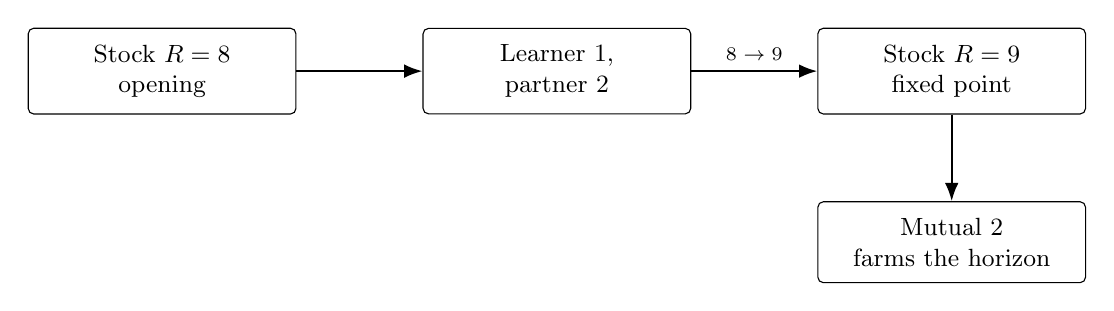
\begin{tikzpicture}[
  box/.style={draw, rounded corners=2pt, align=center, inner sep=6pt,
    font=\small, minimum width=3.4cm},
  arr/.style={-{Latex}, thick},
]
\node[box] (r8) {Stock \(R=8\)\\opening};
\node[box, right=1.6cm of r8] (open) {Learner 1,\\partner 2};
\node[box, right=1.6cm of open] (r9) {Stock \(R=9\)\\fixed point};
\node[box, below=1.1cm of r9] (farm) {Mutual 2\\farms the horizon};
\draw[arr] (r8) -- (open);
\draw[arr] (open) -- node[above, font=\scriptsize] {\(8\to 9\)} (r9);
\draw[arr] (r9) -- (farm);
\end{tikzpicture}
\caption{Basin switch at the opening against a frozen hawk.
  A first-step take of 1 against take-2 moves stock \(8\to 9\).
  At \(R=9\), mutual take-2 is a fixed point and the rest of the horizon
  can be farmed.
  Open 0 against take-2 goes \(8\to 11\), not onto that fixed point.
  A tape of later 2s after open-1 is therefore not evidence of a 36-step
  dove policy.}
\label{fig:farm}
\end{figure}

\section{What is not the live environment}

Linear \(R_0=20\), \(g=2\) is the harvest fixture only.
A retired \(\pm 1\)-on-stock Test~A is archived and is not Stage~B.
Stage~B is the mean-one three-point multiplier on the growth increment
in \eqref{eq:growth}.
The historical park file \texttt{stochastic\_cpr\_env.py} is not the
live game.

\section{Observation surface (prompts)}

\texttt{CPRObservationManager} renders every prompt from structured state.
It never parses a previous prompt string.
Reset observations are
\texttt{game\_description + instruction\_prompt} (rules, Gemma turn tags,
initial resource line at \(R_0\), ``Reply with only one number'').
Subsequent steps add the current resource and a previous-round line that
reports \textbf{requests and receipts} separately, so scarcity is visible.
The shaper, if \texttt{transmit\_info}, also sees joint-request counts and
episode summaries that survive episode boundaries inside a trial and clear
at trial start.
Naive learners reset every episode.
Parallel games render independently.

Integer resource levels only.
Action strings \texttt{"0"}--\texttt{"3"}.

\chapter{Method}
\label{ch:method}

Training reuses the ShapeLLM PPO loop
(\texttt{environment.outer\_rollout}, \texttt{PPOAgent},
\texttt{CustomPPOTrainer}) on the logistic CPR of Chapter~\ref{ch:env}
\cite{garciasegura2025}.
This chapter defines the policy, the reward handed to the optimiser, the
advantage estimator and its two normalisation operators, the PPO objective
with every hyperparameter, and the two training schedules, naive and
shaper, whose difference is the object of Chapter~\ref{ch:results}.
The scientific object is that game's reward, not a new optimiser.

\section{Model, tokens, generation}

Base model: \texttt{google/gemma-2-2b-it}, \texttt{torch.bfloat16}, eager
attention.
Actions are single digit tokens (Table~\ref{tab:tokens}).

\begin{table}[ht]
\centering
\caption{Legal action tokens for Gemma-2-2b-it.
  \texttt{AllowedTokensLogitsProcessor} masks every other vocabulary
  entry.}
\label{tab:tokens}
\begin{tabular}{rr}
\toprule
Action & Token id \\
\midrule
0 & 235276 \\
1 & 235274 \\
2 & 235284 \\
3 & 235304 \\
\bottomrule
\end{tabular}
\end{table}

\paragraph{Policy.}
Each learning agent carries a rank-2 LoRA adapter \(\theta\) on the query
and value projections \cite{hu2022} and a scalar value head
\(V_{\theta}\) on the final hidden state (TRL's
\texttt{AutoModelForCausalLMWithValueHead}); the base weights are frozen.
At round \(t\) the agent receives a prompt \(x_t\) rendered from its
observable history (Chapter~\ref{ch:env}): the rules, the current stock
and, from round~2, the previous round's requests and receipts.
A shaper with \texttt{transmit\_info} also sees the joint-request counts
and episode summaries of the current trial.
The action is one token drawn from the softmax over the four legal action
tokens, every other vocabulary entry being floored by the logits
processor:
\begin{equation}
  \pi_{\theta}(a\mid x_t)
  =
  \frac{\exp z_{\theta}(x_t)_a}{\sum_{a'\in\mathcal{A}}\exp z_{\theta}(x_t)_{a'}},
  \qquad a\in\mathcal{A},
  \label{eq:policy}
\end{equation}
where \(z_{\theta}(x_t)\) are the logits at the answer position.
Generation is one new token (\texttt{max\_new\_tokens=1},
\texttt{do\_sample=True}, \texttt{top\_p=1.0}, \texttt{top\_k=0},
temperature~1), so the emitted token is exactly a draw from
\eqref{eq:policy}.
Illegal draws (observed under MPS multinomial, not under the mask) are
rejection-sampled up to four times.

\paragraph{Untrained prior.}
The pre-flight script (\texttt{scripts/cpr\_preflight.py}) measures the
untrained distribution at about \(0.90\) on token~2.
At the opening prompt of the executed runs, the first episode of every run
(three games before any update) opened 2 on 205 of 240 games, 1 on 25 and
3 on 10, so the untrained opening mass is about \(0.85\) on token~2,
\(0.10\) on token~1, \(0.04\) on token~3 and effectively zero on token~0
(these draws are not independent; see the seeds paragraph below).
That is an executed observation, not a literature citation.
The method does \textbf{not} flatten the prior, does \textbf{not} turn on
\texttt{use\_score\_scaling} / \texttt{use\_score\_norm}, and does
\textbf{not} add a take-1 bonus.
An entropy coefficient of \(0.15\) in early runs bought take-3, not
restraint; all live configurations use \(0.05\), decaying to \(0.01\).

\section{Learning algorithm}
\label{sec:algorithm}

\paragraph{Per-step reward.}
The reward handed to the optimiser at round \(t\) is the receipt
\(c_t\in\{0,1,2,3\}\) of \eqref{eq:harvest}, penalised by the divergence of
the sampled token from the frozen reference model, which is the same
network with the adapter disabled:
\begin{equation}
  \tilde{r}_t
  =
  c_t-\beta_t\bigl[\log\pi_{\theta}(a_t\mid x_t)-\log\pi_{\mathrm{ref}}(a_t\mid x_t)\bigr].
  \label{eq:klreward}
\end{equation}
The coefficient \(\beta_t\) follows the adaptive controller of Ziegler et
al.\ \cite{ziegler2019} as implemented in TRL~0.11.4: initial value
\(0.2\), target divergence \(6\), horizon \(10^{4}\) steps.
With batches of at most \(108\) positions the controller barely moves; the
logged value falls from \(0.200\) to \(0.181\) over the 75 updates of a
15-epoch naive run.
The term is zero under the untrained prior and grows as the policy leaves
it: at \(\pi_{\theta}(1\mid x_1)=0.9\) against \(\pi_{\mathrm{ref}}(1\mid
x_1)=0.1\) it is \(0.2\times\log 9\approx 0.44\) per step, comparable with
the one-unit receipt difference between neighbouring actions.
It is a restoring force towards the prior and is part of every result in
Chapter~\ref{ch:results}.
Steps after collapse (\(R_t=0\)) carry a NaN reward and are dropped from
the batch before any statistic is computed; the collapse step itself is a
real decision and stays.
\texttt{game.records} stores the true zero for those steps.

\paragraph{Advantages.}
Advantages are generalised advantage estimates \cite{schulman2016}
computed by a backward pass over each parallel game,
\begin{equation}
  \delta_t=\tilde{r}_t+\gamma V_{\theta}(x_{t+1})-V_{\theta}(x_t),
  \qquad
  \hat{A}_t=\sum_{l\ge 0}(\gamma\lambda)^{l}\,\delta_{t+l},
  \qquad \gamma=1,\ \lambda=0.97,
  \label{eq:gae}
\end{equation}
where the pass runs over one episode for a naive learner and over the
concatenated episodes of a trial for a shaper, so that with \(\gamma=1\) a
shaper's opening-step advantage includes receipts from later episodes of
the same trial.
The value target is the GAE return \(\hat{G}_t=\hat{A}_t+V_{\theta}(x_t)\).
Before entering the loss, the advantages of a batch \(\mathcal{B}\) are
transformed by one of two operators, where \(\mu_{\mathcal{B}}\) and
\(\sigma_{\mathcal{B}}\) are the mean and standard deviation over the
unmasked positions of the batch:
\begin{equation}
  \mathcal{N}_{\mathrm{whiten}}(\hat{A}_t)
  =
  \frac{\hat{A}_t-\mu_{\mathcal{B}}}{\sqrt{\sigma_{\mathcal{B}}^2+\varepsilon}},
  \qquad
  \mathcal{N}_{\mathrm{centre}}(\hat{A}_t)
  =
  \hat{A}_t-\mu_{\mathcal{B}}.
  \label{eq:norm}
\end{equation}
Whitening is the TRL default (\texttt{masked\_whiten}, the OpenAI
\texttt{lm-human-preferences} convention documented by Huang et al.\
\cite{huang2024}); centring is the \texttt{advantage\_norm=center} flag of
this repository.
Masked positions are zeroed after either operator.
Engstrom et al.\ \cite{engstrom2020} show that PPO's measured behaviour is
driven by such code-level choices, not only by the clip.

\paragraph{Objective.}
With \(\tilde{A}_t=\mathcal{N}(\hat{A}_t)\), the probability ratio
\(\varrho_t=\pi_{\theta}(a_t\mid x_t)/\pi_{\theta_{\mathrm{old}}}(a_t\mid x_t)\),
the old value estimate \(V_{\mathrm{old}}\) and the clipped value
\(V^{\mathrm{c}}=\operatorname{clip}(V_{\theta},V_{\mathrm{old}}-\epsilon_v,V_{\mathrm{old}}+\epsilon_v)\),
each agent maximises the clipped surrogate of Schulman et al.\
\cite{schulman2017}
\begin{equation}
  \begin{aligned}
  \mathcal{L}(\theta)=\mathbb{E}_{\mathcal{B}}\Bigl[
    &\min\bigl(\varrho_t\tilde{A}_t,\;
      \operatorname{clip}(\varrho_t,1-\epsilon,1+\epsilon)\,\tilde{A}_t\bigr)\\
    &-\tfrac{c_v}{2}\max\bigl((V_{\theta}(x_t)-\hat{G}_t)^2,\,(V^{\mathrm{c}}(x_t)-\hat{G}_t)^2\bigr)
    +c_e\,\mathcal{H}\bigl(\pi_{\theta}(\cdot\mid x_t)\bigr)
  \Bigr],
  \end{aligned}
  \label{eq:ppo}
\end{equation}
where the entropy is taken over the four legal tokens only.
The policy clip is \(\epsilon=0.2\) for naive learners (the TRL default;
no live configuration overrides it) and \(0.1\) for the shaper and for
agent~2 of the slow-learning-rate control; the value clip is
\(\epsilon_v=0.2\); \(c_v=0.01\); and \(c_e\) starts at \(0.05\) and falls
by \(0.04/150\) per update with a floor of \(0.01\), so it reaches
\(0.03\) after the 75 updates of a naive run and \(0.046\) after the 15
updates of a shaper.
The optimiser is Adam \cite{kingma2015} with the learning rate of
Table~\ref{tab:hyperparameters} and default moments
(\(\beta_1=0.9\), \(\beta_2=0.999\), \(\varepsilon=10^{-8}\)); one pass
over the batch in minibatches of five; no gradient clipping.
The batch is the set of unmasked positions of one episode (naive) or one
trial (shaper), so its size varies with survival.

\begin{table}[ht]
\centering
\small
\caption{Every hyperparameter of the executed runs.
  ``Shaper'' is agent~2 of the naive--shaper configurations; ``control''
  is agent~2 of the slow-learning-rate naive--naive configuration, which
  copies the shaper's learning rate and clip but keeps the naive schedule
  and prompt.
  Agent~1 of every two-learner configuration, and the learner of Tests
  A~and~B, are naive learners.}
\label{tab:hyperparameters}
\begin{tabularx}{\textwidth}{>{\raggedright\arraybackslash}p{4.3cm}>{\raggedright\arraybackslash}X}
\toprule
Quantity & Value \\
\midrule
Base model & \texttt{gemma-2-2b-it}, bf16, eager attention, base weights frozen \\
Adapter & LoRA \(r=2\), \(\alpha=32\), dropout \(0.05\), on \texttt{q\_proj} and \texttt{v\_proj} \\
Value head & scalar, on the final hidden state \\
Generation & one token, sampling, \texttt{top\_p} 1, \texttt{top\_k} 0, temperature 1 \\
Learning rate (Adam) & naive \(1.41\times 10^{-6}\); shaper \(3\times 10^{-7}\); control \(3\times 10^{-7}\) \\
Adam moments & \(\beta_1=0.9\), \(\beta_2=0.999\), \(\varepsilon=10^{-8}\); no gradient clipping \\
Policy clip \(\epsilon\) & naive 0.2; shaper 0.1; control 0.1 \\
Value clip \(\epsilon_v\), coefficient \(c_v\) & 0.2, 0.01 \\
Entropy coefficient \(c_e\) & \(0.05\to 0.01\), \(-0.04/150\) per update, over the four legal tokens \\
KL coefficient \(\beta_t\) & adaptive, initial 0.2, target 6, horizon \(10^{4}\); logged \(0.200\to 0.181\) over 75 updates \\
\(\gamma\), \(\lambda\) & 1, 0.97 \\
GAE span & naive and control: one episode; shaper: one trial of 5 episodes \\
Update schedule & naive and control: after each episode; shaper: once per trial \\
Batch & unmasked positions of the span (\(\le 108\) per episode, \(\le 540\) per trial) \\
Minibatch, PPO epochs & 5, 1 \\
Trial prompt & shaper only: info-on (counts and episode summaries) or info-off \\
Advantage operator & centre in every two-learner and Stage~B run; whiten in the whitened Test~A/B runs \\
Trial geometry & \(T=36\) rounds, \(E=5\) episodes per trial, 3 parallel games, 15 games per epoch \\
Epochs & 15; 30 for seed-fixed whitened Test~A seed~0; 50 for the long seed-0 runs \\
Updates per 15 epochs & naive and control 75; shaper 15 \\
Seeds & 0, 1, 2 (see the seeds paragraph) \\
Hardware & NVIDIA L40S (RunPod) for Stage~B, the seed-fixed packet, whitened seeds 1--2 and the 50-epoch naive run; Apple silicon (MPS) for the pre-fix Test~A/B seed-0 tapes \\
Software & \texttt{trl} 0.11.4, \texttt{transformers} 4.47.0, \texttt{peft} \\
\bottomrule
\end{tabularx}
\end{table}

\paragraph{Seeds.}
Each experiment \(k\) calls \texttt{set\_seed}\((k)\) before constructing
its agents.
TRL's \texttt{PPOTrainer} then calls \texttt{set\_seed}\((0)\) in its own
constructor (its \texttt{PPOConfig} default), after the adapter and value
head have been created.
On every run dated 6~September or earlier the action sampler was therefore
drawn from the seed-0 stream, and the nominal seed controlled only the
value-head initialisation.
Those runs of nominally different seeds on the same hardware begin
identically and diverge only through non-deterministic bf16 kernels and,
in Stage~B, through the noise tables, which are seeded separately and
correctly.
\texttt{scripts/audit\_seeds\_and\_scale.py} measures the consequence: the
pre-fix whitened Test~A seeds 1 and 2 opened identically on all 75 games
of their first five epochs, and the Stage~B naive--naive, naive--shaper
and slow-LR seeds 1 and 2 opened identically on 92--95\% of games over
the whole run.
The entry points re-seed after construction.
The 8--9~September packet used that fix: seed-fixed Test~A centre pairs
agree on \(0.56\)--\(0.61\) of openings in epochs 1--5 (pre-fix whitened
\(s1\) vs \(s2\) was \(1.00\)); NS~\(\xi\) seed~0 is identical to the
pre-fix seed-0 tape, as expected.
Chapter~\ref{ch:lim} states what this does to the inference.
Write ``three seeds'' for the seed-fixed packet; write ``three nominal
seeds'' for every earlier GPU table.

\section{What the normalisation operator changes}
\label{sec:operator}

The opening-step advantage \(A_0\) is logged for the first index of each
parallel game in the flattened batch, raw and after the operator.
At \(\varrho_t=1\) the policy-gradient term of \eqref{eq:ppo} has expected
gradient on the logit of opening action \(k\)
\begin{equation}
  \frac{\partial\mathcal{L}}{\partial z_k}\Big|_{x_1}
  =
  \pi(k\mid x_1)\bigl(\tilde{A}(k)-\bar{A}\bigr),
  \qquad
  \bar{A}=\sum_{a\in\mathcal{A}}\pi(a\mid x_1)\,\tilde{A}(a),
  \label{eq:logit-update}
\end{equation}
where \(\tilde{A}(a)\) is the normalised opening advantage of action
\(a\), because \(\partial\log\pi(a\mid x)/\partial z_k=\mathbb{1}[a=k]-\pi(k\mid x)\)
for a softmax.
The sign of the update on logit \(k\) is the sign of
\(\tilde{A}(k)-\bar{A}\), so an action whose advantage is positive but
below the policy-weighted mean is pushed down; and the magnitude is
proportional to \(\pi(k\mid x_1)\), so a rare action moves slowly however
large its advantage.
Both operators in \eqref{eq:norm} are affine with positive scale, so they
agree on every sign; they differ in the scale of the gradient by
\(\sigma_{\mathcal{B}}\).

\paragraph{The measured scale.}
Per update, from the \texttt{live\_adv} logs of the six Test~A runs, the
batch standard deviation of the raw advantages has median \(13\)--\(15\)
(interquartile range \(12\)--\(15\) on the centred runs).
On the whitened runs it falls to \(2\)--\(5\) in the updates where every
game collapsed by round~4, because such a batch contains almost no
variation to divide by: whitening then scales an uninformative batch up to
unit variance.
An earlier estimate of \(53\), inferred from run-averaged opening
advantages, was not a per-batch quantity and is withdrawn.

\paragraph{Why the scale is not a step size.}
Adam's update \(\hat{m}/(\sqrt{\hat{v}}+\varepsilon)\) is invariant to a
uniform rescaling of the gradient \cite{kingma2015}, so a run in which
every batch were rescaled by the same \(\sigma_{\mathcal{B}}\) would take
the same steps under either operator.
Multiplying the learning rate by \(\sigma_{\mathcal{B}}\) does not convert
a whitened run into a centred one.
What the operator changes is the weight of the policy-gradient term
relative to two things that are not rescaled.
First, the value loss and the entropy bonus in \eqref{eq:ppo}: under
whitening the policy term is of order one per position while the value
regression on returns of \(10\)--\(100\) contributes a gradient of order
\(c_v\,|V_{\theta}-\hat{G}|\approx 0.01\times 40\) through the shared
adapter, so the two are comparable; under centring the policy term is
\(13\)--\(15\) times larger and dominates.
Second, the other batches: Adam's second moment is a running average over
updates, so the step taken on a batch scales with that batch's gradient
norm relative to the recent history.
Under whitening every batch has unit advantage variance, and a batch in
which every game collapsed drives a step of the same size as a batch
containing a surviving game; under centring the surviving batch carries a
gradient several times larger than a collapse-only batch
(\(\sigma_{\mathcal{B}}\approx 14\) against \(2\)) and takes a
proportionally larger step.
Centring therefore weights informative batches over uninformative ones;
whitening equalises them and raises the relative weight of the critic and
the entropy bonus.
Which of these produced the difference between the whitened and centred
seed-0 runs is not identified by the executed runs; the ablation that
would identify it is whitening with \(c_v\) and \(c_e\) divided by
\(\sigma_{\mathcal{B}}\), or plain SGD in place of Adam, neither of which
was run.

\paragraph{Worked example.}
With the first-episode opening distribution \(\pi(2)\approx 0.85\),
\(\pi(1)\approx 0.10\) and the centred seed-0 opening advantages of
Chapter~\ref{ch:results} (\(\tilde{A}(1)=+16.7\), \(\tilde{A}(2)=-5.7\),
\(\bar{A}\approx -3.2\)), \eqref{eq:logit-update} gives a gradient of
about \(+2.0\) on logit~1 and \(-2.1\) on logit~2.
Dividing by \(\sigma_{\mathcal{B}}\approx 13\) gives the whitened
counterparts \(+0.15\) and \(-0.16\) with the same signs.
The quantity that differed between the whitened seed-0 run and the
whitened seeds 1--2 is not this scale but the sign of
\(\tilde{A}(2)-\bar{A}\): in the seed-0 run the post-operator opening-2
advantage stayed between \(+0.5\) and \(+1.1\) in every epoch because
nearly every game in every batch collapsed, so there was no surviving game
in the batch for the opening-2 games to be compared against, whereas in
seeds 1--2 it turned negative from epoch~4, once surviving games entered
the batches (Table~\ref{tab:a0-epochs}).

\section{Frozen-bot tests (executed path)}

Before any shaper-versus-naive grid, one PPO learner is trained against a
non-learning partner.
This is a \emph{precondition} measurement, not opponent shaping: if the
prior never leaves opening 2 against a partner that is already frozen
on 2, a later two-learner table in which one agent leaves 2 cannot be
read as ``the shaper taught restraint.''
The two-learner and Stage~B grids therefore use mean-centring
(Table~\ref{tab:hyperparameters}), the operator under which leave-2 is
reliable within 15 epochs on this lock.
The TRL default (whitening) is retained as the Test~A/B contrast, not
hidden.

\begin{itemize}
\item \textbf{Test A.} \texttt{ConstantActionAgent} always requests 2
  (frozen hawk).
\item \textbf{Test B.} Same bot always requests 1 (frozen dove).
\end{itemize}

The bot has no Gemma weights.
\texttt{is\_shaper=False} so \texttt{outer\_rollout} calls a no-op
\texttt{update\_parameters} once per episode.
Only the learner's LoRA and value head train.
Records still include both request columns.

Trial geometry in the Test~A/B configs: \(T=36\), \(E=5\)
episodes per trial, \(3\) parallel games, 15 epochs.
That is 15 games per epoch and 225 games per run
(Figure~\ref{fig:trial}).

\begin{figure}[ht]
\centering
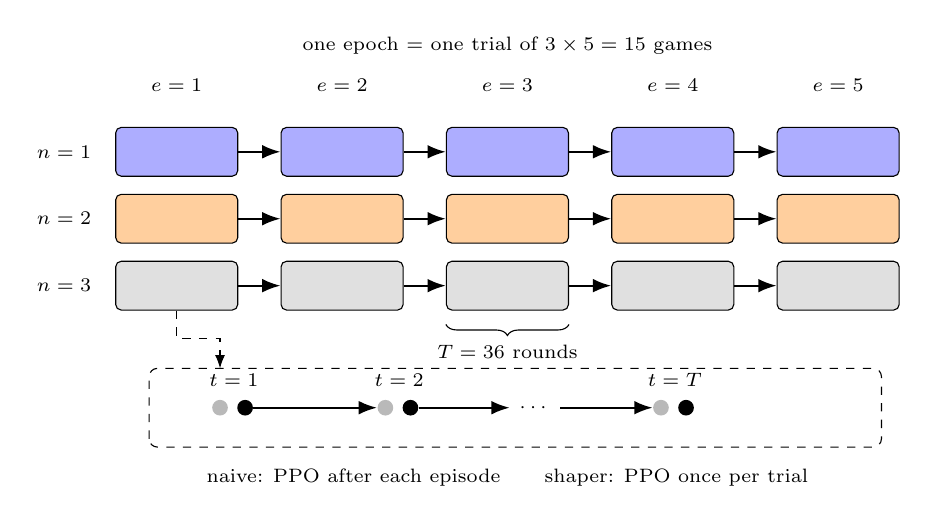
\begin{tikzpicture}[
  font=\small,
  epibox/.style={
    draw, rounded corners=2pt, minimum width=1.55cm,
    minimum height=0.62cm, inner sep=1pt,
  },
  arr/.style={-{Latex}, thick},
  player/.style={circle, inner sep=2.0pt},
]
\node[font=\scriptsize] at (4.2, 3.05)
  {one epoch $=$ one trial of \(3\times 5=15\) games};
\foreach \e/\x in {1/0, 2/2.1, 3/4.2, 4/6.3, 5/8.4} {
  \node[font=\scriptsize] at (\x, 2.55) {$e=\e$};
  \node[epibox, fill=blue!32] (n1e\e) at (\x, 1.70) {};
  \node[epibox, fill=orange!38] (n2e\e) at (\x, 0.85) {};
  \node[epibox, fill=black!12] (n3e\e) at (\x, 0.00) {};
}
\foreach \e in {1,2,3,4} {
  \pgfmathtruncatemacro{\nxt}{\e+1}
  \draw[arr] (n1e\e) -- (n1e\nxt);
  \draw[arr] (n2e\e) -- (n2e\nxt);
  \draw[arr] (n3e\e) -- (n3e\nxt);
}
\node[left=0.18cm of n1e1, font=\scriptsize] {$n=1$};
\node[left=0.18cm of n2e1, font=\scriptsize] {$n=2$};
\node[left=0.18cm of n3e1, font=\scriptsize] {$n=3$};
\draw[decorate, decoration={brace, amplitude=4pt, mirror}]
  ([yshift=-5pt]n3e3.south west) -- ([yshift=-5pt]n3e3.south east)
  node[midway, below=4pt, font=\scriptsize] {$T=36$ rounds};
% one episode, round by round
\node[player, fill=gray!55] (p1a) at (0.55, -1.55) {};
\node[player, fill=black, right=3pt of p1a] (p2a) {};
\node[font=\scriptsize, above=1pt of p1a, xshift=5pt] {$t=1$};
\node[player, fill=gray!55] (p1b) at (2.65, -1.55) {};
\node[player, fill=black, right=3pt of p1b] (p2b) {};
\node[font=\scriptsize, above=1pt of p1b, xshift=5pt] {$t=2$};
\node[font=\scriptsize] (dots) at (4.55, -1.55) {$\cdots$};
\node[player, fill=gray!55] (p1c) at (6.15, -1.55) {};
\node[player, fill=black, right=3pt of p1c] (p2c) {};
\node[font=\scriptsize, above=1pt of p1c, xshift=5pt] {$t=T$};
\draw[arr] (p2a) -- (p1b);
\draw[arr] (p2b) -- (dots);
\draw[arr] (dots) -- (p1c);
\draw[dashed, rounded corners=3pt]
  (-0.35, -2.05) rectangle (8.95, -1.05);
\draw[dashed, -{Latex}] (n3e1.south) -- ++(0,-0.35) -| (0.55, -1.05);
\node[font=\scriptsize, anchor=north] at (4.2, -2.20)
  {naive: PPO after each episode\qquad shaper: PPO once per trial};
\end{tikzpicture}
\caption{One training epoch of the CPR loop, drawn after Garcia Segura
  et al.\ (their Figure~1).
  Rows are three independent parallel copies of the same game.
  Columns are five sequential episodes of \(T=36\) rounds.
  Same-coloured boxes are successive episodes of one parallel copy.
  The dashed box is one episode: both agents act simultaneously each
  round.
  A naive learner updates after every episode; a shaper updates once
  from the whole trial.
  Fifteen such epochs are 225 games.
  Frozen-bot Test~A/B uses the same geometry; the partner does not
  update.}
\label{fig:trial}
\end{figure}

Versus always-2, a constant take-1 scores 36 and lives; constant take-2
scores 7 and dies.
Versus always-1, constant take-2 scores 72 and lives; constant take-1
scores 36; take-3 dies.
Test~B does not treat ``copy 1'' as the unique high-return reply.

\section{Naive and shaping schedules}
\label{sec:schedules}

\texttt{finetuning\_cpr.py} trains two \texttt{PPOAgent}s through the same
\texttt{outer\_rollout}.
Training proceeds in trials of \(E=5\) episodes
(Figure~\ref{fig:trial}).
A naive learner updates its parameters after every episode \(e\) from
that episode's batch,
\begin{equation}
  \theta_{e+1}
  =
  \theta_e+\alpha_{\mathrm{n}}\,\nabla_{\theta}
  \mathcal{L}\bigl(\theta_e;\ \tau_e(\pi_{\theta_e},\pi_{\phi})\bigr),
  \label{eq:naive-update}
\end{equation}
where \(\tau_e\) is the trajectory of episode \(e\) and \(\pi_{\phi}\) is
the partner (the gradient step is Adam's, written here as a plain step for
readability).
A shaper holds \(\phi\) fixed for the whole trial and updates once, from
the concatenated trajectories, towards the model-free opponent-shaping
objective of Lu et al.\ \cite{lu2022} as instantiated for language-model
agents by Garcia Segura et al.\ \cite{garciasegura2025}:
\begin{equation}
  J(\phi)
  =
  \mathbb{E}\Bigl[
    \sum_{e=1}^{E}
    G_{\mathrm{shaper}}^{(e)}\bigl(\pi_{\phi},\pi_{\theta_e}\bigr)
  \Bigr],
  \qquad
  \theta_{e+1}=\theta_e+\alpha_{\mathrm{n}}\nabla_{\theta}
  \mathcal{L}\bigl(\theta_e;\tau_e(\pi_{\theta_e},\pi_{\phi})\bigr).
  \label{eq:shaper-objective}
\end{equation}
The naive objective \eqref{eq:naive-update} treats the partner as fixed
within the episode; the shaper objective \eqref{eq:shaper-objective}
credits \(\phi\) for the partner's parameter change
\(\theta_e\to\theta_{e+1}\) that \(\phi\) induced, through the trial-level
GAE of \eqref{eq:gae}.
That dependence is the only thing that distinguishes shaping from
ordinary learning against a slowly changing opponent, and it can only be
exploited if the shaper's own policy changes on a timescale at which the
naive learner responds.
The shaper's learning rate \(\alpha_{\mathrm{s}}=3\times 10^{-7}\),
tighter clip and once-per-trial schedule therefore also make it a slower,
more stationary opponent than a matched-learning-rate naive learner.
The slow-learning-rate naive--naive control of
Section~\ref{sec:executed-two} gives agent~2 the same learning rate and
clip but the naive schedule and no trial prompt, and so isolates that side
effect from the shaping term.
When \texttt{transmit\_info=true}, the shaper prompt also keeps
joint-request counts and episode summaries for the trial.
Live protocol:
\path{cpr_naive_naive_center.json},
\path{cpr_naive_shaper_center.json},
\path{cpr_naive_shaper_center_info_off.json},
\path{cpr_naive_naive_slow2_center.json}, and their \texttt{\_xi}
counterparts.

\texttt{finetuning\_fixed\_opponent.py} is not used for CPR.

\section{Stage B noise (machinery)}

Stage~B configs (\texttt{cpr\_*\_xi.json}) attach a common-random-number
table of \(\texttt{xi\_tenths}\in\{7,10,13\}\) per seed
(\texttt{cpr\_env.make\_noise\_table}).
The same table is shared across arms so arm contrasts are not confounded
by different draws.
\(\texttt{xi\_tenths}=10\) is bit-identical to Stage~A.
Test~A \(\xi\) uses \texttt{finetuning\_cpr\_fixed.py}; two-learner
\(\xi\) uses \texttt{finetuning\_cpr.py}.
Tables are saved as \texttt{noise\_table.npy} next to the records.
This is a measurement device, not a new optimiser.

\chapter{Implementation}
\label{ch:impl}

The live training path is a duck-typed CPR wrapped onto the unmodified
ShapeLLM rollout.
Logistic growth, the tests and the launcher jointly pin the lock
\(R_0=8\), \(K=40\), \(T=36\), \(\rho=0.9\); the launcher refuses any
other point.
This chapter names the modules an examiner would open, the entry points,
the analysis scripts that produce every number in
Chapters~\ref{ch:design} and~\ref{ch:results}, and the tests that pin
the environment and the estimators.

\section{Modules}

\begin{table}[ht]
\centering
\caption{Load-bearing modules.
  \texttt{verify\_cpr.py} is the linear harvest fixture and is not a
  training environment.}
\label{tab:modules}
\begin{tabularx}{\textwidth}{>{\raggedright\arraybackslash}p{4.6cm}X}
\toprule
Path & Role \\
\midrule
\texttt{cpr\_env.py} & \texttt{CPRDynamics}: integer harvest, scarcity, absorbing zero, logistic growth with \(\xi\); CRN noise tables \\
\texttt{cpr\_game.py} & \texttt{CPRGame}: rollout surface, records, NaN masking of post-collapse steps, noise-table attachment at fixed capacity \\
\texttt{cpr\_observation\_managers.py} & prompts rendered from structured state; trial memory for the shaper \\
\texttt{cpr\_bots.py} & frozen partners: constant action; frozen adapter (transfer arm) \\
\texttt{cpr\_xi.py} & exact dynamic programme: expected values of policy pairs, best response to any fixed policy, joint optimum, under the deterministic, \(\xi\) and binomial kernels \\
\texttt{cpr\_eval.py} & estimators, intervals, paired contrasts, hypothesis readouts, LaTeX emitters \\
\texttt{agents.py}, \texttt{utils/training\_utils.py} & Gemma PPO, legal-token mask, advantage operator, opening and live-advantage logs \\
\texttt{environment.py} & \texttt{inner\_rollout} / \texttt{outer\_rollout}, reused verbatim from ShapeLLM \\
\bottomrule
\end{tabularx}
\end{table}

\section{Entry points and launcher}

\texttt{finetuning\_cpr.py} trains two learners (naive--naive,
slow-LR, info-off, naive--shaper); \texttt{finetuning\_cpr\_fixed.py}
trains one learner against a frozen partner (Tests~A/B, transfer).
Both re-seed after the trainer is constructed
(Chapter~\ref{ch:method}), name experiments by seed, and write the
epoch-1 openings so that seed independence can be checked while a run is
in progress.
Per run they serialise the step records (\(R\), requests, receipts,
collapse, mask), the opening advantages, the live advantages, and the
training statistics; without the records none of the survival or
policy readouts is recoverable.

\texttt{scripts/run\_cpr.sh} asserts \texttt{trl} 0.11.4, runs the
linear fixture and the test suite, checks that the configuration is the
locked logistic point, and launches one configuration; its \texttt{grid}
mode takes the stage, arm, operator and seed from the environment and
\texttt{scripts/launch\_grid.sh} fans seeds out over GPUs.
\texttt{scripts/make\_grid\_configs.py} derives every grid configuration
from the executed Stage~B files so that arms differ in exactly one key.

\section{Analysis scripts}

Every number in the design and results chapters is produced by a script
from the records or the dynamic programme.
\texttt{cpr\_xi.py} prints the values of Tables~\ref{tab:noise-dp}
and~\ref{tab:dp3}.
\texttt{scripts/evaluate\_grid.py} reads one stage of the grid and writes
the per-arm, paired-ladder and \(\hat{\pi}(a\mid R)\) tables, the
learning curves, and a JSON summary of every hypothesis readout;
Chapter~\ref{ch:results} inputs those files.
\texttt{scripts/audit\_seeds\_and\_scale.py} reproduces the seed-identity
and advantage-scale audit; \texttt{scripts/check\_seed\_divergence.py}
is the launch gate; \texttt{scripts/make\_a0\_table.py} produces the
per-epoch opening-advantage table.

\section{Tests}

The suite runs before every launch.
\begin{itemize}
\item \texttt{test\_cpr\_env.py}, \texttt{test\_logistic\_cpr.py},
  \texttt{test\_cpr\_solve.py}: harvest, scarcity, cap-0, exact
  depletion and absorbing zero; half-even rounding; no interior freeze at
  the lock; the constant-pair cells \(36/7/72\).
\item \texttt{test\_cpr\_xi.py}: \(\xi=1\) is bit-identical to Stage~A;
  constant-pair invariance under i.i.d.\ tables; the best-response
  Q-vectors and joint optima of Table~\ref{tab:noise-dp}; the binomial
  kernel's mean identity and broken invariance; noise-table prefix
  invariance across lengths.
\item \texttt{test\_cpr\_eval.py}: every estimator against records
  simulated from policies of known value, the Wilson examples of
  \eqref{eq:wilson}, paired sign agreement, first-majority and
  stationarity, the DP anchors, and the LaTeX emitters.
\item \texttt{test\_cpr\_game.py} and \texttt{test\_cpr\_observations.py}:
  NaN masking against record zeros; prompt rendering.
\item \texttt{test\_opening\_log.py} and \texttt{test\_action\_sampling.py}:
  opening index and the centre/whiten operators; illegal-token redraw.
\end{itemize}
Checkpoints and adapters are not tracked; the experimental record is
\texttt{docs/LIVE\_FACTS.md} and the pre-registration is
\texttt{docs/EXPERIMENT\_PLAN.md}.

\chapter{Experimental design}
\label{ch:design}

This chapter is the pre-registration of the final grid.
Everything in it was fixed before any run of that grid was launched: the
questions, the objects that answer them, the arms, the hypotheses with
their readouts and their nulls, the hyperparameters and what is checked
about them, the protocol, and the rules that decide what happens when a
check fails.
Chapter~\ref{ch:results} reports against this chapter.
The runs executed while the design was being fixed, fifteen epochs each,
are pilots; Section~\ref{sec:pilots} lists the design decisions they
settled and Section~\ref{sec:pilot-results} reports them as pilots.

\section{Questions and the shape of the evidence}
\label{sec:questions}

Three questions, in the order the evidence is built.
\begin{enumerate}
\item \textbf{Structure.} What does the exact solution of the game
  (Chapter~\ref{ch:env}) imply about what a prior-dominated learner can
  learn in it, and in particular whether a shaping objective has anything
  to buy?
  This is answered by dynamic programming before any training run, and it
  is the reason the thesis moves from the deterministic game to
  stochastic regeneration (Section~\ref{sec:a-to-b}).
\item \textbf{Shaping.} Does the trial-level objective of
  \eqref{eq:shaper-objective} change what a naive learner acquires, and
  what the shaper earns, relative to a partner that is merely slow?
  This is answered by an ablation ladder in which one ingredient changes
  per rung (Section~\ref{sec:ladder}).
\item \textbf{Transfer.} Does a trained shaper, frozen, steer a fresh
  learner differently from a frozen hawk?
  This is the claim of Garcia Segura et al.\ \cite{garciasegura2025}
  stated for this game.
\end{enumerate}
The evidence takes one form throughout: an estimated quantity of
\eqref{eq:estimators}, compared with a value fixed in advance by the
dynamic programme or with the same quantity in a paired control, reported
per seed with its interval and summarised across seeds by sign agreement.
With three to five seeds no test statistic is reported; effect sizes
against exact cells are.

\section{From the deterministic game to stochastic regeneration}
\label{sec:a-to-b}

A shaping effect is measured against a counterfactual partner that does
not shape.
Write \(V_{\mathrm{h}}(\sigma)\) for the return of a partner committed to
take-2 when the learner plays \(\sigma\).
The largest effect a shaper can have on its own return is
\begin{equation}
  \Delta^{*}
  =
  V_{\mathrm{h}}(\sigma_{\mathrm{induced}})-V_{\mathrm{h}}(\sigma_{\mathrm{control}}),
  \label{eq:effect-bound}
\end{equation}
the value of the learner policy it can induce minus the value of the
policy the control partner induces.
\eqref{eq:effect-bound} is a bound on power: no experiment can detect an
effect larger than the game offers.

\paragraph{Stage A.}
After any safe opening the learner's best continuation is a constant
action, so the deterministic game is decided in round~1.
A naive learner leaves opening 2 against any hawk on its own
(Section~\ref{sec:pilot-results}), so \(\sigma_{\mathrm{control}}\) already
delivers the hawk its best outcome: \(V_{\mathrm{h}}=72\) against a
partner that restrains at the opening, and \(72\) against a partner that
has learned the feedback rule (Table~\ref{tab:noise-dp}).
The bound \eqref{eq:effect-bound} is at most one unit.
A null in Stage~A is therefore uninformative about the objective, and a
positive result in Stage~A would be an artefact.
Hypothesis H-A below tests this prediction with the same arms as Stage~B,
which makes the move from A to B a result of the thesis rather than an
assumption of it.

\paragraph{Stage B.}
Under the multiplier \(\xi_t\) of \eqref{eq:growth} the continuation is
a decision (Section~\ref{sec:noise-arm}).
A hawk earns \(72\) against a partner that plays the feedback rule
``1 if \(R<12\), else 2'', \(35.7\) against a partner that restrains only
at the opening, and \(7.4\) against mutual take-2, all exact
(Table~\ref{tab:noise-dp}).
If the naive learner does not acquire the feedback rule on its own, the
bound is \(72-35.7=36.3\) on the hawk's side; if the shaper does more
than commit to take-2 and exploits a partner it has taught to restrain,
the best response to the feedback rule is \(105.5\)
(Table~\ref{tab:dp3}), so the bound is \(69.8\).
Whether the learner acquires the rule alone is check C2 below; the bound
that applies to H-B is conditional on it.
The learner's own stake is of the same size (\(68.8\) against \(34.7\),
survival \(1.00\) against \(0.40\)), so both parties gain from the
feedback rule and the question is whether the shaping objective supplies
what a slow partner does not.

\paragraph{Estimators.}
An epoch is \(n=15\) games.
For agent \(i\), opening leave-2, survival, mean return, and
stock-conditioned action frequency in an epoch are
\begin{equation}
  \begin{aligned}
  \hat{L}_i
  &=
  \frac{1}{n}\sum_{j=1}^{n}\mathbb{1}\bigl[a^{(j)}_{i,1}\ne 2\bigr],
  &\quad
  \hat{S}
  &=
  \frac{1}{n}\sum_{j=1}^{n} S^{(j)},
  \\
  \hat{G}_i
  &=
  \frac{1}{n}\sum_{j=1}^{n} G_i^{(j)},
  &\quad
  \hat{\pi}_i(a\mid R)
  &=
  \frac{\sum_{j,t}\mathbb{1}[R^{(j)}_t=R,\,a^{(j)}_{i,t}=a]}
       {\sum_{j,t}\mathbb{1}[R^{(j)}_t=R]}.
  \end{aligned}
  \label{eq:estimators}
\end{equation}
Last-three-epoch quantities pool \(n=45\).
The tables write those estimators in shorthand a cold reader can decode
without the laboratory:
\begin{itemize}
\item \textbf{Last-open.} Counts of the 15 first-round harvests in
  epoch~15. \(10\times 0+5\times 1\) means ten of those games opened 0
  and five opened 1, not ten epochs of 0.
\item \textbf{Last surv / last ret.} \(\hat{S}\) and \(\hat{G}\) on
  those same 15 games. Stay-on-2 against a hawk returns about 7 and
  dies around round~4; open-1-then-2s returns 71 on the deterministic
  lock.
\item \textbf{Leave-2 last3.} \(\hat{L}\) pooled over epochs 13--15
  (45 openings).
\item \textbf{First majority.} First epoch with \(\hat{L}>8/15\).
\end{itemize}
The opening is round~1 of a 36-round game. Later tokens on a surviving
tape are not last-open.

For a count \(k\) out of \(n\), the \(95\%\) Wilson interval is
\begin{equation}
  \frac{\hat{p}+z^2/2n \;\pm\; z\sqrt{\hat{p}(1-\hat{p})/n+z^2/4n^2}}{1+z^2/n},
  \qquad \hat{p}=k/n,\ z=1.96,
  \label{eq:wilson}
\end{equation}
so \(13/15\) is \([0.62,0.96]\), \(9/15\) is \([0.36,0.80]\) and
\(15/15\) is \([0.80,1.00]\).
Seeds are the unit of replication.
Runs dated 6~September or earlier shared one action-sampling stream
(Chapter~\ref{ch:method}); the 8--9~September packet re-seeds after
agent construction and is three independent seeds on L40S.
Every contrast between configurations is reported as the per-seed
difference and its sign across seeds.
In Stage~B the noise table at a given (epoch, game, round) is identical
across configurations for the same seed, so a between-arm difference on
seed \(s\),
\begin{equation}
  \Delta_s(\hat{Y})=\hat{Y}^{(\mathrm{arm}\,1)}_s-\hat{Y}^{(\mathrm{arm}\,2)}_s,
  \label{eq:paired}
\end{equation}
is a paired comparison in which the environmental draws cancel; with
three seeds, agreement of the sign of \(\Delta_s\) across all seeds is
reported rather than a test statistic.


Per-epoch series of the same quantities are the learning curves; the
window statistics are taken over the last \(W=20\) epochs of a run
(\(W=3\) for the fifteen-epoch pilots).
Two derived quantities describe the dynamics: the first epoch at which a
share exceeds one half (first majority), and stationarity, defined as the
last-window mean differing from the preceding-window mean by less than
the pooled standard error.
Every estimator is implemented in \texttt{cpr\_eval.py} and tested
against records simulated from policies of known value
(\texttt{tests/test\_cpr\_eval.py}) before it is applied to a training
run.

\section{Arms and the ablation ladder}
\label{sec:ladder}

Agent~1 is always a naive learner with the hyperparameters of
Table~\ref{tab:hyperparameters}.
The arms differ in agent~2 (Table~\ref{tab:arms}) and are run in both
stages with the same seeds and, in Stage~B, the same noise tables.

\begin{table}[ht]
\centering
\small
\caption{Arms of the final grid.
  Each rung of the ladder from naive--naive to naive--shaper changes one
  ingredient of agent~2; the configuration files differ in exactly the
  key named in the last column
  (\texttt{scripts/make\_grid\_configs.py}).}
\label{tab:arms}
\begin{tabularx}{\textwidth}{l>{\raggedright\arraybackslash}p{4.6cm}X}
\toprule
Arm & Agent 2 & Isolates (key that changes) \\
\midrule
Test A & frozen always-2 & what a naive learner can learn against a perfectly stationary hawk; the ceiling for C2 \\
naive--naive & naive, learning rate \(1.41\times 10^{-6}\), clip 0.2 & symmetric baseline: who restrains, whether coordination breaks under \(\xi\) \\
slow-LR & naive, learning rate \(3\times 10^{-7}\), clip 0.1 & stationarity of the partner alone (\texttt{learning\_rate}, \texttt{cliprange}) \\
info-off shaper & trial objective \eqref{eq:shaper-objective}, no trial prompt & the trial-level objective (\texttt{is\_shaper}) \\
naive--shaper & trial objective and trial prompt & the trial prompt (\texttt{transmit\_info}) \\
transfer & frozen epoch-100 shaper adapter & whether the trained shaper's policy steers a fresh learner (Stage~B only) \\
\bottomrule
\end{tabularx}
\end{table}

The rung slow-LR to info-off is the test of the objective itself: learning
rate, clip and prompt are equal and only the once-per-trial update with
trial-level advantages differs.
Without it the contrast naive--shaper against slow-LR cannot separate
the objective from the prompt.
The cell ``trial prompt without trial objective'' is not run; if H-B3 is
positive and H-B2 null it becomes the follow-up.

\section{Hypotheses}
\label{sec:hypotheses}

All quantities are last-window estimates of \eqref{eq:estimators};
\(\hat{L}_i(R<12)\) is leave-2 restricted to unmasked rounds with
\(0<R_t<12\); superscripts A and B denote the stage; \(s\) indexes seeds;
\(\Delta_s\) is the paired difference \eqref{eq:paired} between the arms
named.
Two checks precede the hypotheses.
\begin{align}
  \text{C1 (opening invariance):}\quad
  & \hat{L}^{\mathrm{B}}_{1}(s)\in
    \mathrm{CI}_{95}\bigl(\hat{L}^{\mathrm{A}}_{1}(s)\bigr)
    \ \text{ for each } s \text{ (Test~A)},
  \label{eq:c1}\\[3pt]
  \text{C2 (learnability):}\quad
  & \hat{L}^{\mathrm{B}}_{1}(R<12)\ge 0.5
    \ \text{ and }\
    \widehat{\Pr}(S=1\mid a_{1,1}\ne 2)\ge 0.40 .
  \label{eq:c2}
\end{align}
C1 says the noise did not change the opening incentive, which the
dynamic programme predicts (Table~\ref{tab:noise-level}); a shift from
opening 1 to opening 0 within leave-2 is consistent with it, since
\(Q(0)>Q(1)\).
C2, evaluated on Stage~B Test~A, says a naive learner can acquire
stock-conditioned restraint against a stationary hawk within the
horizon; the constants are the
constant-continuation survival cell and a majority of low-stock rounds.
The hypotheses follow.
\begin{align}
  \text{H-A:}\quad
  & \bigl|\Delta_s(\hat{G}_2)\bigr|\le 1
    \ \text{ and }\ \Delta_s(\hat{L}_1)\in\mathrm{CI}_{95}
    \quad\text{for every } s \ \text{(Stage~A)},
  \label{eq:ha}\\[3pt]
  \text{H-B}k\text{:}\quad
  & \Delta^{(k)}_s(\hat{G}_2)>0
    \ \text{ and }\ \Delta^{(k)}_s\bigl(\hat{L}_1(R<12)\bigr)>0
    \quad\text{for every } s,\ k\in\{1,2,3\} \ \text{(Stage~B)},
  \label{eq:hb}\\[3pt]
  \text{H-B4:}\quad
  & \hat{G}^{\mathrm{shaper}}_{2}(s)-1.96\,\widehat{\mathrm{se}}
    > 72 \quad\text{for every } s,
  \label{eq:hb4}\\[3pt]
  \text{H-T:}\quad
  & \Delta^{(\mathrm{T})}_s\bigl(\hat{L}_1(R<12)\bigr)>0
    \ \text{ and }\ \Delta^{(\mathrm{T})}_s(\text{first majority})<0
    \quad\text{for every } s.
  \label{eq:ht}
\end{align}
H-A is the contrast naive--shaper minus slow-LR in Stage~A.
The rungs \(\Delta^{(k)}_s\) are \(k=1\): slow-LR minus naive--naive
(stationarity); \(k=2\): info-off minus slow-LR (trial objective);
\(k=3\): naive--shaper minus info-off (trial prompt); the overall
contrast naive--shaper minus slow-LR is reported alongside.
H-B4 compares the shaper's return with the plain-hawk cell \(72\) and
reads the excess against the ceiling \(105.5\).
\(\Delta^{(\mathrm{T})}_s\) is the fresh learner against the frozen
shaper minus the same learner against the frozen hawk.
Survival and the first-majority epoch of low-stock restraint are reported
for every rung as secondary readouts.

\paragraph{Nulls.}
For H-A the null is the prediction: no rung in Stage~A moves the shaper's
return by more than the one-unit bound.
For H-B\(k\) the null is a mixed sign of \(\Delta_s\) across seeds or a
mean below the sampling interval; the effect size is reported against the
bound of Section~\ref{sec:a-to-b} whichever way it falls.
For H-B4 the null is a shaper return inside the interval of the plain-hawk
cell, which means the shaper committed to take-2 and nothing more.
For H-T the null is no difference between the frozen shaper and the
frozen hawk in what the fresh learner acquires.
A null on any hypothesis is reported as a null with its effect size; none
is rescued by a secondary readout.

\section{Stage B: multiplicative noise on the growth increment}
\label{sec:noise-arm}


The deterministic lock limits what a shaping experiment on it can show.
Against a near-constant partner the fate of the pool is decided by the
joint opening: first-round \((1,2)\) moves stock \(8\to 9\), from which
mutual take-2 is a fixed point; first-round \((2,2)\) leaves the stock at
8 and mutual take-2 collapses around round~4.
Opening 0 versus a hawk moves stock \(8\to 11\), not onto that fixed
point (Chapter~\ref{ch:env}).
After a safe opening, a constant continuation needs no stock information.
A hawk in a hawk--dove split gains one unit (72 against 71) from its
partner's restraint.
Stage~B multiplies the locked growth increment by a mean-one three-point
shock so that the continuation, not only the opening, is a decision
problem.
The deterministic increment is the mean of a per-unit Bernoulli regrowth
process, the scalar form of the density-dependent respawn of Commons
Harvest \cite{perolat2017}; the multiplier is a bounded, mean-preserving
discretisation of that process's spread, chosen so that the constant-pair
cells of Table~\ref{tab:chicken} keep their deterministic values, which
the exact per-unit process does not (Appendix~\ref{app:binomial}).
In the terms of Reed \cite{reed1979} and Sethi et al.\ \cite{sethi2005}
the arm studies growth uncertainty alone, with the shock on the surplus
rather than on the whole recruitment so that collapse remains
attributable to harvest; the joint optimum and the safe feedback rules
below are constant-escapement policies in Reed's sense
(Appendix~\ref{app:reed}).

\subsection{Form}

Let \(R_t\) be the post-harvest stock in round \(t\).
The Chapter~\ref{ch:env} update is
\(R_{t+1}=\min\bigl(K,\, R_t + g_t(R_t)\bigr)\) with
\begin{equation}
  g_t(R)
  \;=\;
  \mathrm{round\_half\_even}\bigl(
    \xi_t\,\rho\, R\,(K-R)/K
  \bigr),
  \qquad
  \xi_t\in\{0.7,\,1.0,\,1.3\}
  \text{ equally likely},
  \label{eq:noise-update}
\end{equation}
\(\rho=0.9\).
The multiplier has mean one, bounded support, and is applied to the
growth increment only.
The post-harvest stock is never perturbed.
In code the multiplier is \(\texttt{xi\_tenths}\in\{7,10,13\}\) inside the
integer Fraction
\(9\,\xi\,R\,(K-R)/(100K)\).
\(\texttt{xi\_tenths}=10\) is bit-identical to Stage~A.
\(\xi\) is never applied at post-harvest \(R=0\).
Draws are independent across rounds and across parallel games, and are
shared by both players within a game.
A discrete support keeps the state space finite (41 stocks, 36 rounds,
three draws), so the game is solved exactly by dynamic programming
(\texttt{cpr\_xi.py}) rather than estimated by simulation.

\subsection{Level and invariance}

The level \(\pm 30\%\) is the largest symmetric three-point multiplier at
which the constant-pair survival cells of Table~\ref{tab:chicken} are
unchanged.
Under hawk versus dove the post-harvest stock is 5 and deterministic
growth is \(3.94\to 4\); with multiplier \(0.7\) the growth is
\(2.76\to 3\), exactly the joint harvest, so the pairing remains safe.
Under mutual take-2 from \(R_0=8\) the post-harvest stock is 4 and
deterministic growth is \(3.24\to 3\); with multiplier \(1.3\) the growth
is \(4.21\to 4\), returning the stock to 8, so the profile never reaches
the fixed point at 9.
(The all-\(\xi=1.3\) sequence is a live 8-cycle; under i.i.d.\ draws that
path has probability \(3^{-36}\).)
At \(\pm 40\%\) both bounds fail: multiplier \(1.4\) lifts mutual take-2
to 9 with positive probability, and multiplier \(0.6\) drives hawk--dove
below 8.
Table~\ref{tab:noise-level} records the i.i.d.\ survival probabilities.

\begin{table}[ht]
\centering
\caption{Survival probability to the horizon for constant action pairs
  and for open-1-then-2s, as a function of the three-point noise level.
  Exact dynamic-programming values from \texttt{cpr\_xi.py}.
  \(\pm 30\%\) leaves the constant-pair cells of Table~\ref{tab:chicken}
  unchanged; larger levels do not.
  The mutual take-2 entry at \(\pm 30\%\) is not exactly zero
  (\(P<10^{-15}\)).}
\label{tab:noise-level}
\begin{tabular}{lcccc}
\toprule
Noise level & \((1,1)\) & \((2,2)\) & \((2,1)\) & open 1 then 2s \\
\midrule
deterministic & 1.00 & 0.00 & 1.00 & 1.00 \\
\(\pm 30\%\)  & 1.00 & 0.00 & 1.00 & 0.80 \\
\(\pm 40\%\)  & 1.00 & 0.15 & 0.83 & 0.78 \\
\(\pm 50\%\)  & 1.00 & 0.15 & 0.84 & 0.67 \\
\bottomrule
\end{tabular}
\end{table}

Invariance of the constant-pair cells is the design property that makes
Stage~B comparable with Stage~A.
The opening decision faces the same constant-pair incentives in both
arms.
Opening values against a frozen always-2 partner, then best-response
continuation, are \(Q=(105,104,102,6)\) in the deterministic game and
\(Q=(102.5, 101.7, 99.1, 91.1)\) under \(\pm 30\%\) noise, for openings
\(0,1,2,3\).
Same ordering on \(0,1,2\); the gap between openings 1 and 2 is \(2.0\)
and \(2.6\) respectively.
Opening 3 then best-response continuation is \(91.1\) under noise because
a stock-conditioned continuer can recover; that is not the untrained
prior.

\subsection{Structure of the stochastic game}

What the noise changes is the continuation.
Under mutual take-2 the stock is a random walk with three regions:
from \(R\ge 11\) the minimum draw returns the stock to at least 11, so
mutual take-2 is safe for the rest of the horizon;
from \(R\le 7\) collapse is certain within a few rounds;
and \(R\in\{8,9,10\}\) is a gamble.
The deterministic fixed point at 9 lies inside the gamble region.
A first \((1,1)\) or \((0,2)\) places the stock in \(\{9,11,12\}\), so
open-0-then-2s against a hawk survives with probability \(0.80\)
(learner return \(58.3\)); a first \((1,2)\) places it in
\(\{8,9,10\}\), so open-1-then-2s against a hawk survives with
probability \(0.40\) (learner return \(34.7\)).
The rule ``take 1 if \(R<12\), else take 2'' survives with probability
one against a frozen hawk (return \(72/68.8\)).
The rule ``take 3 if \(R\ge 14\), else take 0'' survives with probability
one and returns \(102.7\) per player when both use it.
Table~\ref{tab:noise-dp} collects the values.

\begin{table}[ht]
\centering
\caption{Expected return per player and survival probability for
  representative policies in the deterministic game and under
  \(\pm 30\%\) multiplicative noise.
  Exact dynamic-programming values from \texttt{cpr\_xi.py}, rounded to
  one decimal except \((2,2)=7.44\).
  ``Hawk'' is the frozen always-2 partner of Test~A.
  The first three rows are the constant-pair cells and are invariant.
  Every ``good opening, then constant action'' policy becomes risky under
  noise; stock-conditioned feedback rules remain safe.}
\label{tab:noise-dp}
\resizebox{\textwidth}{!}{%
\begin{tabular}{lcccc}
\toprule
 & \multicolumn{2}{c}{Deterministic} & \multicolumn{2}{c}{\(\pm 30\%\) noise} \\
\cmidrule(lr){2-3}\cmidrule(lr){4-5}
Policy pair & Return & Survival & Return & Survival \\
\midrule
\((1,1)\) throughout & 36 / 36 & 1.00 & 36.0 / 36.0 & 1.00 \\
\((2,2)\) throughout & 7 / 7 & 0.00 & 7.44 / 7.44 & 0.00 \\
\((2,1)\) hawk versus dove & 72 / 36 & 1.00 & 72.0 / 36.0 & 1.00 \\
\midrule
\((1,1)\) once, then \((2,2)\) & 71 / 71 & 1.00 & 59.3 / 59.3 & 0.80 \\
Hawk versus ``1 once, then 2'' & 72 / 71 & 1.00 & 35.7 / 34.7 & 0.40 \\
Hawk versus ``0 once, then 2'' & 72 / 70 & 1.00 & 60.3 / 58.3 & 0.80 \\
\((0,0)\) once, then \((3,3)\) & 105 / 105 & 1.00 & 38.7 / 38.7 & 0.25 \\
\midrule
Hawk versus ``1 if \(R<12\), else 2'' & 72 / 69 & 1.00 & 72.0 / 68.8 & 1.00 \\
Both ``2 if \(R\ge 9\), else 1'' & 71 / 71 & 1.00 & 70.8 / 70.8 & 1.00 \\
Both ``3 if \(R\ge 14\), else 0'' & 105 / 105 & 1.00 & 102.7 / 102.7 & 1.00 \\
\midrule
Best response to hawk & 105 & 1.00 & 102.5 & 1.00 \\
Symmetric joint optimum (per player) & 105 & 1.00 & 103.3 & 1.00 \\
\bottomrule
\end{tabular}%
}
\end{table}

Two rows of Table~\ref{tab:noise-dp} define the stakes for the shaping
question.
A hawk that commits to take-2 obtains 72 if its partner uses the
feedback rule and 35.7 if its partner restrains only in round~1; in the
deterministic game the corresponding figures are 72 and 72.
The noise therefore creates a 36-unit interest, on the part of a
committed hawk, in its partner's stock-conditioned restraint, where the
deterministic game offered none, and the partner's cost of providing that
restraint relative to its deterministic return is about two units
(68.8 against 71).
A shaper that did more than commit to take-2 could do better still: the
best response to a partner playing the feedback rule is \(105.5\) under
noise (\(107\) deterministic), so the ceiling on what a shaper gains from
a partner it has taught to restrain is \(105.5\) against the \(72\) of a
plain hawk (Table~\ref{tab:dp3}).
These values are from \texttt{cpr\_xi.py}.


\section{Hyperparameters and sensitivity}
\label{sec:sensitivity}

Table~\ref{tab:hyperparameters} lists every hyperparameter.
Table~\ref{tab:provenance} states where each came from, because several
that earlier drafts described as inherited from ShapeLLM are not: the
released ShapeLLM configurations use an entropy coefficient of zero and
a value coefficient of \(0.1\) for two learners, and a clip of \(0.1\), a
value coefficient of \(0.01\) and a KL coefficient of \(2.0\) with target
\(1\) for a learner against a fixed opponent.

\begin{table}[ht]
\centering
\small
\caption{Provenance of the hyperparameters.
  ``Ours'' means chosen in this project; the sensitivity column names the
  alternative value checked in Section~\ref{sec:sensitivity}.}
\label{tab:provenance}
\begin{tabularx}{\textwidth}{>{\raggedright\arraybackslash}p{2.7cm}>{\raggedright\arraybackslash}p{3.6cm}>{\raggedright\arraybackslash}p{2.6cm}X}
\toprule
Parameter & ShapeLLM release & Live value & Status; sensitivity check \\
\midrule
Naive learning rate & \(1.41\times 10^{-6}\) & \(1.41\times 10^{-6}\) & inherited \\
Shaper learning rate & not released & \(3\times 10^{-7}\) & ours; \(1.41\times 10^{-6}\) \\
Policy clip & 0.2 (two learners), 0.1 (fixed opponent) & 0.2 naive, 0.1 shaper & mixed inheritance \\
Value coefficient \(c_v\) & 0.1 (two learners), 0.01 (fixed opponent) & 0.01 & taken from the fixed-opponent file; 0.1 \\
Entropy coefficient & 0 & \(0.05\to 0.01\) & ours (a pilot at 0.15 bought take-3); 0 \\
KL coefficient & 2.0, target 1 (fixed opponent); default otherwise & 0.2, target 6 (TRL default) & differs; 2.0 with target 1 \\
\(\gamma\), \(\lambda\) & defaults & 1, 0.97 & ours \\
Minibatch & 10 / 6 & 5 & ours \\
Advantage operator & whitening (TRL default) & whitening & inherited; centring in the pilots \\
\bottomrule
\end{tabularx}
\end{table}

A full sweep is neither affordable nor what the argument needs.
The parameters marked ours or mixed are checked one at a time from the
live setting on the cheapest arm that exercises the learner, Stage~B
Test~A, one seed, the full epoch budget: entropy \(0\) against
\(0.05\); \(c_v=0.1\) against \(0.01\); the ShapeLLM fixed-opponent KL
setting against the TRL default; and the shaper learning rate
\(1.41\times 10^{-6}\) against \(3\times 10^{-7}\) on the naive--shaper
arm, because that is the shaper's own parameter and the timescale
confound is this thesis's concern.
The readout is the C2 triple (low-stock restraint, conditional survival,
return).
The result is reported as one table with the statement that the
learnability result is or is not sensitive to each parameter; the grid is
not rerun on that basis unless a setting flips C2, in which case rule R3
below applies.

\section{Protocol}
\label{sec:protocol}

\paragraph{Seeds and platform.}
Three seeds per arm, five on the Stage~B ladder where the thesis claim
lives.
Every run on one NVIDIA L40S; the Apple-silicon pilots are not results,
because bf16 kernels differ between backends and the seed audit of
Chapter~\ref{ch:method} showed platform-dependent divergence.
The entry points re-seed after the trainer is constructed, so seeds are
independent draws; the first epoch of seeds 0 and 1 is compared before
any arm continues and the launch stops if their openings are identical.

\paragraph{Length.}
Every arm runs 100 epochs (1{,}500 games, 500 naive updates, 100 shaper
updates), with the stationarity criterion of Section~\ref{sec:questions}
evaluated over epochs 81--100.
Paired arms share a length: if the naive--shaper arm is not stationary on
any seed, naive--shaper and slow-LR are extended together to 200 on all
seeds.
The Stage~B noise tables are generated at 200 epochs for every seed and
sliced, so an extension keeps the draws of its first 100 epochs and every
arm sees the same draw at the same (epoch, game, round)
(\texttt{tests/test\_cpr\_xi.py}).

\paragraph{Transfer.}
The epoch-100 adapter of each naive--shaper seed is saved; a fresh naive
learner is trained against it, frozen, for 30 epochs, with the shaper's
own prompt rendered as in training, and compared with Stage~B Test~A.

\paragraph{Decision rules.}
R1: Stage~A Test~A with whitened advantages launches first; if any seed's
last-window leave-2 share is below one half, the grid runs with centred
advantages and the operator contrast returns as a result.
R2: the length rule above.
R3: if C2 fails on every seed, H-B is read against the
constant-continuation cell (\(35.7\)) rather than the feedback cell
(\(72\)), and the shaping question becomes whether the shaper makes the
learner acquire what it could not acquire alone.

\paragraph{Budget.}
Measured on the L40S, one two-learner epoch costs about 50 seconds and
one Test~A epoch about 20 seconds.
Stage~B (Test~A, four ladder arms, transfer) at three seeds is about
20 GPU-hours; Stage~A the same without transfer; the sensitivity block
five hours; two further seeds on the Stage~B ladder eight hours.
On five GPUs the whole grid is one working day.

\paragraph{Readouts.}
\texttt{scripts/evaluate\_grid.py} reads the records of every arm and
writes, per stage, the per-arm table of last-window estimates with
intervals, the paired ladder table with sign agreement, \(\hat{\pi}_1(a\mid
R)\) over the last window per arm, and the learning curves; the tables in
Chapter~\ref{ch:results} are those files.

\section{Pilot runs and the decisions they fixed}
\label{sec:pilots}

Fifteen-epoch runs were executed while the design was being fixed:
Tests A and B against frozen bots, the four two-learner arms in Stage~A
and Stage~B, two 50-epoch single-seed extensions, and, after the seed fix,
Test~A under both operators and the Stage~B naive--shaper and slow-LR
arms with independent seeds.
They are reported in Section~\ref{sec:pilot-results} as pilots.
They fixed five decisions.
An entropy coefficient of \(0.15\) moved the learner onto take-3 rather
than restraint; \(0.05\) is used.
Centred advantages left opening 2 within 15 epochs and whitened advantages
did so on a slower, more variable schedule (locking from epoch 23 on a
30-epoch seed); the grid uses the TRL default with rule R1.
The seed audit showed the nominal seeds shared one sampling stream; the
entry points were fixed and the seed-fixed pilots confirmed independent
divergence.
With independent seeds the 15-epoch contrast naive--shaper against
slow-LR had mixed sign on every readout, where the shared-stream pilots
had agreed on every seed; that is why the grid runs 100 epochs and five
seeds on that contrast.
The mixed Apple-silicon and L40S provenance of the early pilots is why the
grid runs on one platform.

\chapter{Results}
\label{ch:results}

This chapter has two parts.
Section~\ref{sec:pilot-results} reports the fifteen-epoch pilot runs
that fixed the design (Section~\ref{sec:pilots}); their numbers are
correct records of what happened but their seeds, platforms and lengths
are those of pilots, and no claim of the thesis rests on them alone.
Section~\ref{sec:grid-results} reports the final grid against the
hypotheses of Section~\ref{sec:hypotheses}.

\section{Pilot runs}
\label{sec:pilot-results}

\subsection{Executed runs}
\label{sec:executed-fixed}

\subsubsection{Test A, whitened (\texttt{advantage\_norm=whiten})}

Config: \path{configs/cpr_testA_always2.json}.
Partner: frozen always-2.
Folders: \path{checkpoints/cpr_log_testA_always2} (run) and
\path{checkpoints/cpr_log_testA_a0} (same Test~A with opening A0
logged --- the A0 photograph).

Outcomes:
\begin{itemize}
\item Opening-step critic: raw A0 \(\mathbf{+39.8}\) on 1 versus
  \(\mathbf{+6.2}\) on 2.
\item After batch whitening, A0 \(\mathbf{+1.38}\) versus
  \(\mathbf{+0.75}\).
\item Policy still peaked on 2.
  Take-1 live-step \(\mathbf{6\% \to 3\%}\).
  Survival \(\mathbf{28/225}\).
\item Open-1 share: about \(\mathbf{27\%}\) floor, falling
  (epoch \(1 \to 15\)).
\item Take-1 live-step at epoch 15: \(\mathbf{3\%}\).
\end{itemize}

Read \textbf{openings}, not only live-step mix: after a first 1,
\(R\colon 8\to 9\) and \((2,2)\) is a fixed point, so a surviving policy
can be mostly 2s on the tape while every game opened 1.

\subsubsection{Test B, whitened}

Config: \texttt{configs/cpr\_testB\_always1.json}.
Partner: frozen always-1.
Opening A0 also logged (\texttt{testB\_a0}).

Outcomes: survival \(\mathbf{219/225}\); opening 1 and opening 2 received
the same star; mix \(\mathbf{80\% \to 38\%}\) on 2,
\(\mathbf{18\% \to 62\%}\) on 3.

Versus a dove, constant-2 pays 72 and lives; constant-1 pays 36.
There is no 64-versus-7 basin that would force copy-1.

\subsubsection{Test A, centered (\texttt{advantage\_norm=center})}

Config: \texttt{configs/cpr\_testA\_center.json}.
Same seed family as whitened Test~A.
Mean-subtract, no \texttt{/std}.
Folder: \texttt{checkpoints/cpr\_log\_testA\_center}.
15 epochs, frozen always-2.

Table~\ref{tab:whiten-vs-center} is the whitened-versus-centre contrast on
that seed family.

\begin{table}[ht]
\centering
\small
\caption{Test~A outcomes under batch whitening versus centre-only
  advantages (same seed family, frozen always-2).
  Open-1 share is the primary readout; live-step take-1 is not.}
\label{tab:whiten-vs-center}
\begin{tabularx}{\textwidth}{>{\raggedright\arraybackslash}p{3.4cm}XX}
\toprule
 & Whitened Test A & Center Test A \\
\midrule
Take-1 live-step, epoch 15 & 3\% & 9\% \\
Open-1 share, epoch \(1 \to 15\) &
  \(\sim 27\%\) floor, falling &
  \(\mathbf{27\% \to 87\%}\) (100\% at epoch 12) \\
Survival & 28/225 &
  epoch 1: 2/15; epoch 12: \(\mathbf{15/15}\); epoch 15: 13/15 \\
Open-1 A0 (what PPO saw) & +1.38 whitened &
  \(\mathbf{+16.7}\) centered (raw still \(\sim +40\)) \\
Open-2 A0 & +0.75 & \(\mathbf{-5.7}\) \\
\bottomrule
\end{tabularx}
\end{table}

Later 2s still have large \emph{raw} GAE (smear).
After centering they sit near 0; openings of 1 do not.

Run extras: take-3 live-step \(\mathbf{8.5\% \to 0\%}\); survival
\(\mathbf{134/225}\); last three epochs \(\mathbf{41/45}\) openings were
1.

\subsubsection{Test B, centered}

Config: \path{configs/cpr_testB_center.json}.
Folder: \path{checkpoints/cpr_log_testB_center}.
Frozen always-1, seed 0.

Outcomes: survival \(\mathbf{223/225}\); live mix \(\mathbf{98\%}\) on 2;
open-1 share \(\mathbf{13\% \to 13\%}\) (2/15 last epoch).
Did not copy-1.
Opening A0 on 1 and 2 both large and similar (centred \(\sim +20\) /
\(+22\)).

\subsubsection{Test A center, extra seeds}

Folder: \texttt{checkpoints/cpr\_log\_testA\_center\_s12}
(\texttt{exp1\_} seed 1, \texttt{exp2\_} seed 2).

\begin{itemize}
\item Seed 1: open-1 \(\mathbf{27\% \to 93\%}\), survival
  \(\mathbf{113/225}\), last epoch 14/15 opened 1.
\item Seed 2: open-1 \(\mathbf{27\% \to 7\%}\), survival
  \(\mathbf{160/225}\), last epoch \(\mathbf{14/15}\) opened 0.
\end{itemize}

Same center flag, same frozen hawk.
Heterogeneity is a recorded outcome, not a claim.
These extra seeds are the pre-fix family (shared sampling stream;
Chapter~\ref{ch:method}).

\subsubsection{Seed-fixed Test A, centre and whitened (8--9 Sep, all L40S)}

After the trainer reseed fix.
Configs \path{configs/cpr_testA_center.json} and
\path{configs/legacy/cpr_testA_always2.json}.
Folders \path{checkpoints/cpr_log_testA_center_reseed} and
\path{checkpoints/cpr_log_testA_whiten_reseed}, three seeds \(\times\) 15
epochs; plus whitened seed~0 for 30 epochs
(\path{checkpoints/cpr_log_testA_whiten_reseed_e30}).

Identity of agent-1 openings in epochs 1--5: centre pairs \(0.56\)--\(0.61\),
whitened pairs \(0.63\) (pre-fix whitened \(s1\) vs \(s2\) was \(1.00\)).
Outcomes are in Chapter~\ref{ch:results}.
Table shorthand (last-open, last surv, last ret, leave-2 last3, first
majority) is defined at the start of this chapter: last-open is the 15
first-round harvests of epoch 15, not a count of epochs.
Do not call epoch 15 an endpoint: the 30-epoch whitened seed~0 is the
continuation of the 15-epoch snapshot.

Figure~\ref{fig:openings} plots the first-to-last open-1 share for
whitened Test~A and the three centred seeds, using only those endpoint
numbers.

\begin{figure}[ht]
\centering
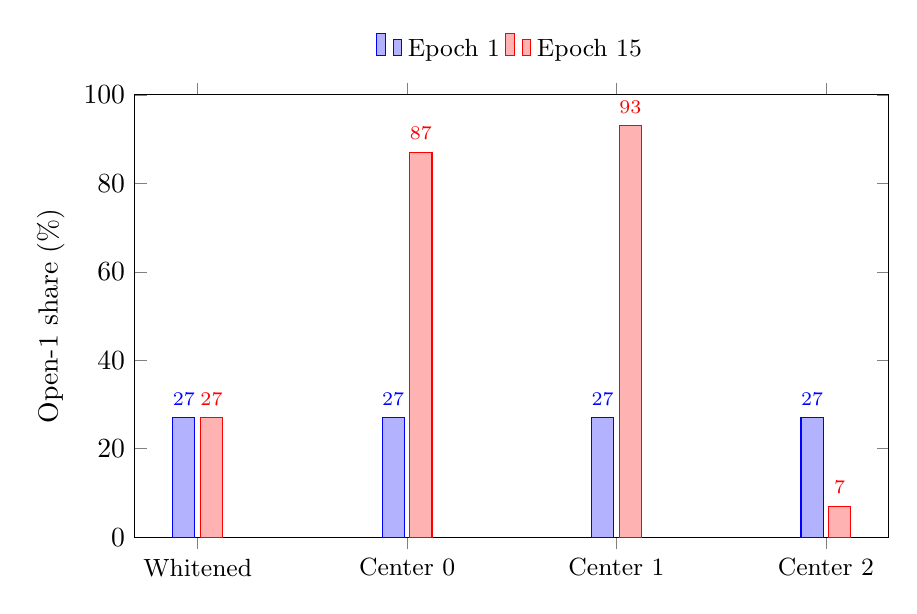
\begin{tikzpicture}
\begin{axis}[
  ybar,
  bar width=8pt,
  width=0.92\textwidth,
  height=7.2cm,
  ylabel={Open-1 share (\%)},
  ymin=0, ymax=100,
  symbolic x coords={Whitened, Center 0, Center 1, Center 2},
  xtick=data,
  xticklabel style={font=\small},
  legend style={at={(0.5,1.05)}, anchor=south, legend columns=2,
    font=\small, draw=none},
  nodes near coords,
  nodes near coords style={font=\scriptsize, /pgf/number format/fixed},
  every node near coord/.append style={yshift=1pt},
]
\addplot coordinates {(Whitened,27) (Center 0,27) (Center 1,27) (Center 2,27)};
\addplot coordinates {(Whitened,27) (Center 0,87) (Center 1,93) (Center 2,7)};
\legend{Epoch 1, Epoch 15}
\end{axis}
\end{tikzpicture}
\caption{Test~A open-1 share at the first and last epoch against a frozen
  hawk.
  Whitened last-epoch share is not recorded as a separate number; the
  executed note is a \(\sim 27\%\) floor, falling, so the last bar repeats
  that floor rather than inventing a lower point.
  Centre seeds~0 and~1 rise to \(87\%\) and \(93\%\).
  Centre seed~2 falls to \(7\%\) (last epoch almost all opening~0, not~1).
  Survival: whitened \(28/225\); seeds \(0/1/2\): \(134/225\),
  \(113/225\), \(160/225\).}
\label{fig:openings}
\end{figure}

\subsection{Executed runs --- two learners}
\label{sec:executed-two}

Same lock, \texttt{advantage\_norm=center}, entropy 0.05.
Claim statistic: share of episodes that do \textbf{not} open 2.
Do not put unmatched epoch lengths in one versus-naive table.

\subsubsection{Centred naive--naive, 15 epochs, seeds 0--2}

Config \path{configs/cpr_naive_naive_center.json}.
Folders \path{checkpoints/cpr_log_naive_naive_center} (seed 0) and
\path{checkpoints/cpr_log_naive_naive_center_s12} (seeds 1--2).

\begin{table}[ht]
\centering
\small
\caption{Centred naive--naive, 15 epochs.
  Who leaves opening 2 swaps across seeds.
  Live mix at epoch 15 is still mostly 2s on the tape.}
\label{tab:nn}
\begin{tabular}{llll}
\toprule
 & Seed 0 & Seed 1 & Seed 2 \\
\midrule
Surv e1 / e15 & 2/15 / 15/15 & 2/15 / 13/15 & 2/15 / 14/15 \\
Survived & 119/225 & 98/225 & 115/225 \\
A1 last openings & \(15\times 0\) & \(9\times 1\), \(5\times 2\), \(1\times 3\) &
  \(1\times 0\), \(8\times 1\), \(6\times 2\) \\
A2 last openings & \(3\times 1\), \(12\times 2\) &
  \(1\times 0\), \(14\times 1\) & \(13\times 1\), \(2\times 2\) \\
A1 leave-2 first3\(\to\)last3 & \(11\%\to 96\%\) & \(7\%\to 53\%\) &
  \(7\%\to 64\%\) \\
A2 leave-2 first3\(\to\)last3 & \(11\%\to 29\%\) & \(16\%\to 84\%\) &
  \(20\%\to 84\%\) \\
\bottomrule
\end{tabular}
\end{table}

\subsubsection{Centred naive--shaper, three seeds by 15 epochs}

Config \path{configs/cpr_naive_shaper_center.json}.
Folder \path{checkpoints/cpr_log_naive_shaper_center}.
Agent 2: trial update, LR \(3\times 10^{-7}\), \texttt{cliprange=0.1},
extra trial prompt on.

\begin{table}[ht]
\centering
\small
\caption{Centred naive--shaper, 15 epochs.
  Who leaves 2 did not swap: agent 1 dove, agent 2 hawk on all three seeds.}
\label{tab:ns}
\begin{tabular}{llll}
\toprule
 & Seed 0 & Seed 1 & Seed 2 \\
\midrule
Surv e15 & 13/15 & 9/15 & 13/15 \\
Survived & 113/225 & 120/225 & 100/225 \\
A1 last openings & \(1\times 0\), \(13\times 1\), \(1\times 2\) &
  \(1\times 0\), \(14\times 1\) & \(7\times 0\), \(8\times 1\) \\
A2 last openings & \(14\times 2\), \(1\times 3\) &
  \(2\times 1\), \(9\times 2\), \(4\times 3\) & \(14\times 2\), \(1\times 3\) \\
A1 / A2 leave-2 last3 & \(96\%\) / \(0\%\) & \(93\%\) / \(7\%\) &
  \(87\%\) / \(2\%\) \\
A2 leave-2 whole run & 5\% & 5\% & 4\% \\
\bottomrule
\end{tabular}
\end{table}

\subsubsection{Shaper 50 epochs, seed 0}

Folder \path{checkpoints/cpr_log_naive_shaper_center_e50}.
Compare to naive at epoch 15 only.

Epoch 15: 13/15 survived, agent 1 \(13\times 1\), agent 2 \(14\times 2\).
Epoch 50: 15/15, agent 1 \(15\times 1\), agent 2 \(15\times 2\).
Whole run 572/750.
Agent 2 opened 0 or 1 on 25/750 (3.3\%).
No epoch with agent-2 leave-2 majority.

\subsubsection{Info-off shaper, three seeds by 15 epochs}

Config \path{configs/cpr_naive_shaper_center_info_off.json}.
Trial update and LR unchanged; \texttt{transmit\_info=false}.

\begin{table}[ht]
\centering
\small
\caption{Centred naive--shaper with \texttt{transmit\_info=false}.
  Who leaves 2 did not swap.
  Agent-2 leave-2 over the whole run is 16--19\% versus 4--5\% with the
  extra prompt.}
\label{tab:infooff}
\begin{tabular}{llll}
\toprule
 & Seed 0 & Seed 1 & Seed 2 \\
\midrule
Surv e15 & 14/15 & 13/15 & 14/15 \\
Survived & 118/225 & 107/225 & 89/225 \\
A1 last openings & \(14\times 0\) & \(1\times 0\), \(14\times 1\) &
  \(14\times 0\), \(1\times 1\) \\
A2 last openings & \(13\times 2\) & \(12\times 2\) & \(12\times 2\) \\
A1 / A2 leave-2 last3 & \(96\%\) / \(18\%\) & \(89\%\) / \(22\%\) &
  \(89\%\) / \(13\%\) \\
A2 leave-2 whole run & 16\% & 19\% & 16\% \\
\bottomrule
\end{tabular}
\end{table}


\subsubsection{Protocol (as executed)}

Four centred configurations, \(\xi\) on, no other change:
Test~A against a frozen hawk, naive--naive, naive--shaper, and slow-LR
naive--naive, each three seeds \(\times\) 15 epochs of 15 games.
Advantages are mean-centred.
The batch-whitened variant is not repeated on this arm.
The 6~September packet is the pre-fix family (shared seed-0 action
stream).
The 8--9~September packet repeats naive--shaper \(\xi\) and slow-LR
\(\xi\) after the fix, plus a 50-epoch slow-LR \(\xi\) seed~0; Test~A
\(\xi\) and naive--naive \(\xi\) were not repeated; naive--shaper
\(\xi\) at 50 epochs was not obtained (OOM).
A 30-epoch whitened Test~A (deterministic, not \(\xi\)) is in the
seed-fixed Test~A subsection.
The rules text was left unchanged: it does not state a regeneration
schedule, the stock is reported every round, and the unused prompt
clause \texttt{XI\_GROWTH\_CLAUSE} was not spliced in.

For each seed a table of shape (epochs, games, rounds) is drawn once
from a dedicated seed sequence (\texttt{cpr\_env.make\_noise\_table}),
stored as \texttt{noise\_table.npy}, and loaded by every configuration
on the arm.
The draw at a given (epoch, game, round) is therefore identical across
the four arms for the same seed, and independent of any action taken.
That is a measurement device, not a new algorithm
\cite{piche2025}.

Exact checks live in \texttt{tests/test\_cpr\_xi.py}: mean-one
multiplier; \(\xi=1.0\) bit-identical to Stage~A; constant-pair
invariance under i.i.d.\ tables; absorbing zero.

Folders (pre-fix):
\path{checkpoints/cpr_log_testA_center_xi},
\path{checkpoints/cpr_log_naive_naive_center_xi},
\path{checkpoints/cpr_log_naive_shaper_center_xi},
\path{checkpoints/cpr_log_naive_naive_slow2_center_xi}.
Folders (seed-fixed):
\path{checkpoints/cpr_log_naive_shaper_center_xi_reseed},
\path{checkpoints/cpr_log_naive_naive_slow2_center_xi_reseed},
\path{checkpoints/cpr_log_naive_naive_slow2_center_xi_reseed_e50}.
A retired \(\pm 1\)-on-stock Test~A is archived; those numbers are not a
Results table.

\begin{table}[ht]
\centering
\small
\caption{Stage~B GPU, three \emph{nominal} seeds \(\times\) 15 epochs
  (pre-fix, shared action stream).
  Report against Table~\ref{tab:noise-dp}, not only against each other.
  Seed-fixed NS and slow2 are Table~\ref{tab:stageb-reseed}.
  Interpretation is in Chapter~\ref{ch:results}.}
\label{tab:stageb}
\begin{tabular}{lp{3.4cm}p{7.4cm}}
\toprule
Arm & Survived (s0/s1/s2) & Leave-2 last3 \\
\midrule
Test~A \(\xi\) & 119, 41, 93 / 225 &
  98\%, 64\%, 98\%.
  Last openings \(15\times 0\) / \((10\times 1+5\times 2)\) / \(15\times 0\). \\
NN \(\xi\) & 100, 43, 82 / 225 &
  who-doves mixed (seed~2 a2 87\% leave-2; seed~1 both mostly 2) \\
NS \(\xi\) & 90, 71, 75 / 225 &
  a1 96/93/89\%; a2 0/11/11\% hawk \\
slow2 \(\xi\) & 53, 44, 39 / 225 &
  a2 last3 18/18/20\%; last epoch 12--13\(\times 2\) \\
\bottomrule
\end{tabular}
\end{table}

\begin{table}[ht]
\centering
\small
\caption{Stage~B GPU after the trainer reseed fix, three independent
  seeds \(\times\) 15 epochs, all L40S.
  Seed~0 of each arm is the pre-fix seed-0 tape.
  Test~A \(\xi\) and NN \(\xi\) were not repeated.
  Report against Table~\ref{tab:noise-dp}.}
\label{tab:stageb-reseed}
\begin{tabular}{lp{3.4cm}p{7.4cm}}
\toprule
Arm & Survived (s0/s1/s2) & Leave-2 last3 \\
\midrule
NS \(\xi\) reseed & 90, 44, 29 / 225 &
  a1 96/44/33\%; a2 0/22/22\%.
  Last3 surv \(36/45\), \(12/45\), \(5/45\). \\
slow2 \(\xi\) reseed & 53, 61, 34 / 225 &
  a1 69/76/27\%; a2 18/13/22\%.
  Last3 surv \(21/45\), \(24/45\), \(8/45\). \\
slow2 \(\xi\) e50 s0 & 443/750 &
  last-open a1 \(15\times 0\); a2 mixed \(6\times 1+8\times 2+1\times 3\);
  last ret \(70.5/69.2\). \\
\bottomrule
\end{tabular}
\end{table}



These first runs are \textbf{learner versus a frozen constant partner} on the
locked logistic chicken (\(R_0=8\), \(K=40\), \(T=36\),
\texttt{rate\_tenths=9}).
Two-learner numbers follow in Section~\ref{sec:twolearners}; they are not
licensed as ``shaping works.''
Gemma-2-2b-it starts with a strong take-2 prior.
Centre-only advantages (\texttt{advantage\_norm=center}: mean-subtract, no
\texttt{/std}) are the update used in the centred runs.
Default TRL \texttt{masked\_whiten} (batch mean and divide-by-std) is the
whitened contrast.
That difference is an implementation default, not a PPO-paper axiom.

\subsection{What a claim is allowed to use}

Mutual take-2 from \(R=8\) dies around round~4.
A first-step take of \textbf{1} against a take-2 partner moves stock
\(8\to 9\).
At \(R=9\), mutual take-2 is a fixed point and the rest of the horizon can
be farmed.
A first-step take of \textbf{0} against take-2 moves stock \(8\to 11\),
not onto that fixed point.
The opening statistic still counts leave-2 (open 0 or 1).
Those two tokens are not the same basin.

Statistics, decoded for a reader who has not sat the runs
(Chapter~\ref{ch:design} writes the same quantities as
\(\hat{L}\), \(\hat{S}\), \(\hat{G}\)):

\begin{itemize}
\item \textbf{Primary.} Share of episodes that do not open 2 (open 1 or
  open 0). Each epoch is 15 games (5 episodes \(\times\) 3 parallel
  games). The opening is round~1 of each 36-round game.
\item \textbf{Last-open.} The 15 first-round harvests in epoch~15.
  \(10\times 0+5\times 1\) is ten games that opened 0 and five that
  opened 1, not ten epochs.
\item \textbf{Last surv / last ret.} How many of those 15 games reached
  \(T=36\), and the mean learner return on them.
  Stay-on-2 against a hawk is about 7; open-1-then-2s is 71
  deterministic.
\item \textbf{Leave-2 last3.} Leave-2 share over epochs 13--15 (45
  games).
\item \textbf{First majority.} First epoch in which leave-2 exceeded
  \(8/15\).
\item \textbf{Supporting.} Whole-run survival and death round.
\item \textbf{Not the claim.} Live-step action mix.
  After a good opening, a tape of 2s is the \(R=9\) farm.
\end{itemize}

Raw opening advantage already starred that basin.
Under whitening the star was compressed until the prior won on count.

\subsection{Test A --- frozen hawk (always 2)}

\textbf{Whitened.}
Live take-1 fell \(6\%\to 3\%\).
Survival was \(28/225\); deaths around round~4.
Raw opening A0 was about \(+39.8\) on open 1 versus \(+6.2\) on open 2.
After whitening those became \(+1.38\) versus \(+0.75\).
Sign survived; scale did not.

\textbf{Centre-only, seed 0.}
Survival \(134/225\).
Open-1 share \(27\%\to 87\%\); last epoch \(13/15\) opened 1 (from
\(4/15\)).
Epoch 12 was \(15/15\) open 1 and \(15/15\) survived.
Centred opening A0 stayed loud on 1 (\(+16.7\) versus \(-5.7\) on 2; raw on
1 still \(\sim +40\)).
Later 2s in winning games centre near 0: the jackpot stays on the first
step.
Take-3 died (\(8.5\%\to 0\%\)).
Live mix remains mostly take-2 after the opening because that is the
fixed-point farm.

\textbf{Seeds 1 and 2.}
Leaving opening 2 replicates; the restraint \emph{token} need not
(Table~\ref{tab:seeds}).

\begin{table}[ht]
\centering
\caption{Last-epoch openings and run survival for centred Test~A against a
  frozen hawk (pre-fix family, shared sampling stream).
  Seed~2 last epoch is almost all opening~0, not~1.}
\label{tab:seeds}
\begin{tabular}{lll}
\toprule
Seed & Last-epoch openings & Survived \\
\midrule
0 & \(13/15\) opened 1 & \(134/225\) \\
1 & \(14/15\) opened 1 & \(113/225\) \\
2 & \(14/15\) opened 0, one opened 1 & \(160/225\) \\
\bottomrule
\end{tabular}
\end{table}

Seed 2 last epoch left opening 2 via \textbf{0} (\(14/15\)), not 1.
That is leave-2 on the primary statistic.
It is not the \(R=8\to 9\) farm (open 0 vs hawk goes \(8\to 11\)).
Stage~A opening values against a hawk are \(Q(0)=105\) and \(Q(1)=104\),
so both tokens leave 2; the token is not identified by that one-unit gap.

\textbf{Whitened extra seeds (RNG 1--2).}
Seed 0 staying on 2 is not the whole family.
Seed 1 last epoch opened 1 on \(15/15\) (leave-2 last3 \(87\%\), survival
\(97/225\), return \(69.5\)).
Seed 2 last epoch opened 0 on \(12/15\) and 1 on \(3/15\) (leave-2 last3
\(82\%\), survival \(80/225\), return \(69.7\)).
Both extra seeds survived \(15/15\) in the last epoch.

\textbf{Pre-fix family (shared sampling stream).}
Against a frozen hawk, centre-only advantages moved the policy off
opening 2 on three \emph{nominal} seeds.
Batch whitening did that on seeds 1--2 and did not on seed 0
(survival \(28/225\), last epoch \(14\times 2\); that seed-0 tape is MPS).
Treated as a binary leave-2 outcome at three nominal seeds each, the
operators are not distinguishable (whitened \(1/3\) stayed on 2, centred
\(0/3\)).
They differ by the factor \(1/\sigma_{\mathcal{B}}\) in \eqref{eq:norm},
with \(\sigma_{\mathcal{B}}\) measured per update at \(13\)--\(15\)
(Section~\ref{sec:operator}); under Adam that factor is a reweighting of
the policy gradient against the critic, the entropy bonus and the other
batches, not a larger step.
What separates the pre-fix whitened run that stayed on opening 2 from the
five that left it is visible in the opening advantages themselves
(Table~\ref{tab:a0-epochs}): in that MPS seed 0 the post-operator
advantage of opening 2 stayed between \(+0.5\) and \(+1.1\) in every
epoch, because nearly every game in every batch collapsed and there was
no surviving game for the opening-2 games to be compared against, so by
\eqref{eq:logit-update} logit 2 was never pushed down; in whitened seeds
1--2 and in every centred run it turned negative by epoch 4 once
surviving games entered the batches.

\textbf{Seed-fixed Test A, all L40S, \(3\times 15\).}
After the trainer reseed fix the three seeds are independent
(opening identity epochs 1--5 is \(0.56\)--\(0.63\); pre-fix whitened
\(s1\) vs \(s2\) was \(1.00\)).
Centre-only left opening 2 on all three seeds
(Table~\ref{tab:seeds-reseed}): first leave-2 majority at epochs 7, 7, 8;
last-epoch openings \(10\times 0+5\times 1\), \(14\times 0+1\times 1\),
\(14\times 1+1\times 2\); last-epoch survival \(14/15\), \(15/15\),
\(11/15\); last-epoch return \(67.1\), \(80.7\), \(59.1\); leave-2 last3
\(93\%\), \(98\%\), \(91\%\).
Whitened is slower and more seed-variable: leave-2 last3 \(31\%\),
\(96\%\), \(71\%\); first majority at epochs 15, 7, 13; last-epoch
survival \(5/15\), \(13/15\), \(9/15\); last-epoch return \(34.7\),
\(62.4\), \(42.3\); seed 0 last epoch mixed \(8\times 1+7\times 2\).
It is not ``fails to leave'': two of three last epochs have leave-2
majority.

\textbf{Whitened 30 epochs, seed 0.}
Epoch 15 matches the 15-epoch snapshot (survival \(5/15\), return
\(34.7\), leave-2 \(8/15\)).
Leave-2 then stalls through epoch 21 and locks from epoch 23
(\(12/15\) open 1).
Last epoch \(15\times 1\), survival \(13/15\), last3 survival \(42/45\),
return \(64.5\).
Do not call epoch 15 an endpoint.

\textbf{Claim.}
Against a frozen hawk, with independent seeds on the same GPU,
centre-only advantages left opening 2 on three seeds by epoch 8.
Whitening left on a longer and more variable schedule.
The prior yields on the first action when it leaves 2.
It does not become a habit of take-1 across the tape.
Do not write that whitening always keeps the death-open.
Do not treat a 15-epoch last-epoch binary as the operator contrast.
This is a precondition finding: it says whether the prior can leave 2
against a statue that already plays hawk, which operator does so within
the 15-epoch budget used later, and that two-learner runs therefore use
mean-centring.
It is not opponent shaping, and it is not tested off Gemma-2-2b-it on
this lock.

\begin{table}[ht]
\centering
\small
\caption{Opening advantages by epoch for the six Test~A runs against the
  frozen hawk.
  \(k\) is the number of the 15 games that did not open 2;
  \(\tilde{A}(\ne 2)\) and \(\tilde{A}(2)\) are the mean post-operator
  opening advantages of the games that opened 0 or 1 and of the games
  that opened 2 (a dash means no game opened that way).
  Whitened values are in units of the batch standard deviation; centred
  values are in units of return.
  Generated by \texttt{scripts/make\_a0\_table.py} from the
  \texttt{opening\_a0} logs.}
\label{tab:a0-epochs}
\resizebox{\textwidth}{!}{\begin{tabular}{lrrrrrrrrrrrrrrr}
\toprule
 & \multicolumn{3}{c}{Epoch 1} & \multicolumn{3}{c}{Epoch 4} & \multicolumn{3}{c}{Epoch 8} & \multicolumn{3}{c}{Epoch 12} & \multicolumn{3}{c}{Epoch 15} \\
\cmidrule(lr){2-4} \cmidrule(lr){5-7} \cmidrule(lr){8-10} \cmidrule(lr){11-13} \cmidrule(lr){14-16}
Run & $k$ & $\tilde A(\ne 2)$ & $\tilde A(2)$ & $k$ & $\tilde A(\ne 2)$ & $\tilde A(2)$ & $k$ & $\tilde A(\ne 2)$ & $\tilde A(2)$ & $k$ & $\tilde A(\ne 2)$ & $\tilde A(2)$ & $k$ & $\tilde A(\ne 2)$ & $\tilde A(2)$ \\
\midrule
Whitened, seed 0 & 5 & +1.3 & +1.0 & 2 & +1.4 & +0.6 & 3 & +1.3 & +0.6 & 3 & +1.3 & +0.6 & 1 & +1.5 & +1.1 \\
Whitened, seed 1 & 3 & +1.6 & +0.4 & 6 & +1.4 & -0.3 & 10 & +1.2 & -0.3 & 10 & +1.3 & -0.9 & 15 & +1.5 & -- \\
Whitened, seed 2 & 3 & +1.5 & +0.3 & 6 & +1.3 & -0.4 & 5 & +1.3 & -0.4 & 7 & +1.4 & +0.1 & 15 & +1.3 & -- \\
Centred, seed 0 & 5 & +9.2 & +0.8 & 4 & +18.8 & -5.5 & 12 & +17.2 & -16.0 & 15 & +17.6 & -- & 13 & +20.2 & -17.6 \\
Centred, seed 1 & 5 & +9.8 & +1.1 & 9 & +14.3 & -12.2 & 14 & +9.3 & -14.8 & 15 & +13.7 & -- & 14 & +16.1 & -20.5 \\
Centred, seed 2 & 5 & +8.6 & -0.1 & 7 & +17.2 & -15.2 & 14 & +11.4 & -17.3 & 15 & +14.8 & -- & 15 & +17.8 & -- \\
\bottomrule
\end{tabular}
}
\end{table}

\begin{table}[ht]
\centering
\small
\caption{Seed-fixed Test~A against a frozen hawk, all L40S, 15 epochs.
  One learner, not two; the partner is frozen always-2.
  Last-open is the 15 first-round harvests of epoch~15
  (\(10\times 0+5\times 1\) = ten opened 0, five opened 1).
  Last surv / ret are survival and mean return on those 15 games.
  Leave-2 last3 is the leave-2 share over epochs 13--15 (45 games).
  First majority is the first epoch with leave-2 \(>8/15\).
  Identity of openings in epochs 1--5 is \(0.56\)--\(0.63\) between seeds
  (pre-fix whitened \(s1\) vs \(s2\) was \(1.00\)).}
\label{tab:seeds-reseed}
\begin{tabular}{llll}
\toprule
 & s0 & s1 & s2 \\
\midrule
Centre last-open & \(10\times 0,5\times 1\) & \(14\times 0,1\times 1\) & \(14\times 1,1\times 2\) \\
Centre last surv / ret & \(14/15\), \(67.1\) & \(15/15\), \(80.7\) & \(11/15\), \(59.1\) \\
Centre leave-2 last3 & \(93\%\) & \(98\%\) & \(91\%\) \\
Centre first majority & 7 & 7 & 8 \\
Whitened last-open & \(8\times 1,7\times 2\) & \(13\times 1,2\times 0\) & \(7\times 1,3\times 0,5\times 2\) \\
Whitened last surv / ret & \(5/15\), \(34.7\) & \(13/15\), \(62.4\) & \(9/15\), \(42.3\) \\
Whitened leave-2 last3 & \(31\%\) & \(96\%\) & \(71\%\) \\
Whitened first majority & 15 & 7 & 13 \\
\bottomrule
\end{tabular}
\end{table}

\begin{figure}[ht]
\centering
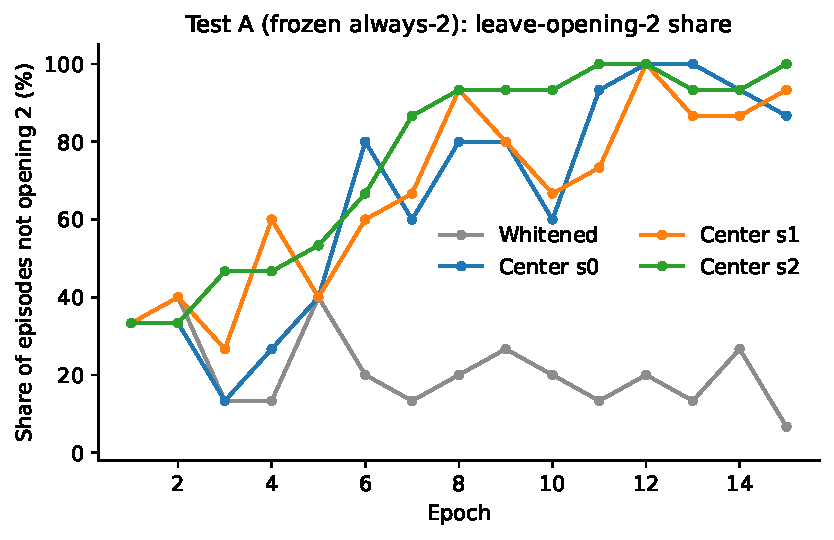
\includegraphics[width=0.92\textwidth]{figures/fig_openings_testA.pdf}
\caption{Share of episodes that do not open 2 (open 0 or 1) against a
  frozen always-2 partner.
  Pre-fix family: the whitened curve is MPS seed~0, which stays on the
  death-open; whitened seeds 1--2 left opening 2 (text).
  Centre-only seeds 0--2 leave opening 2.
  Seed-fixed all-L40S numbers are Table~\ref{tab:seeds-reseed}.
  Seed~2's last epochs leave 2 mostly via opening~0, not 1
  (Table~\ref{tab:seeds}): leave-2, not the \(R=9\) farm.
  This figure is the opening statistic.
  It is not a 36-step dove policy and not a shaping result.}
\label{fig:openingsA}
\end{figure}

\begin{figure}[ht]
\centering
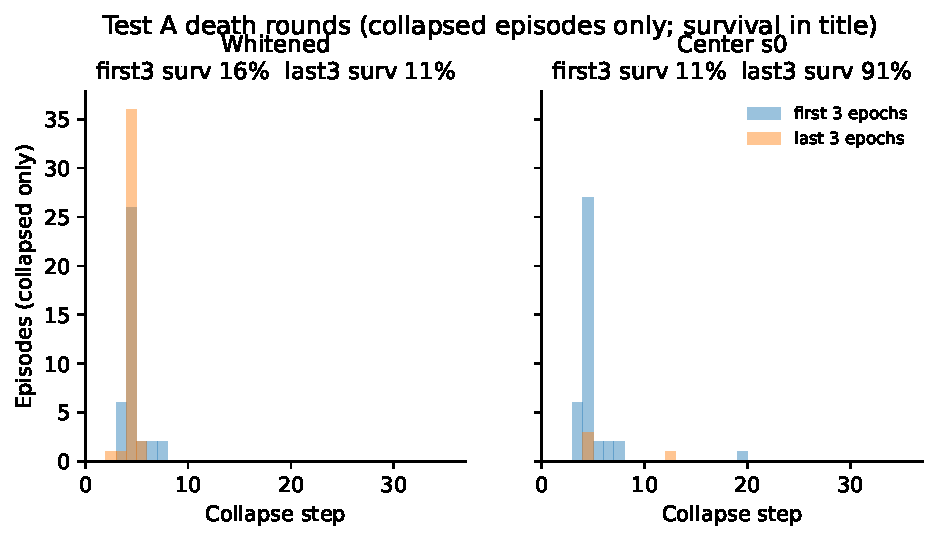
\includegraphics[width=0.92\textwidth]{figures/fig_death_rounds_testA.pdf}
\caption{Collapse step among episodes that die, first three versus last
  three epochs of Test~A.
  Pre-fix family: the whitened panel is MPS seed~0, which keeps dying
  near round~4.
  Centre-only seed~0 last epochs mostly survive (survival in the panel
  titles).
  Supporting statistic only; the claim is the opening share in
  Figure~\ref{fig:openingsA}.}
\label{fig:deathsA}
\end{figure}

The live-step mix at epoch 15 is still mostly 2s under centre (take-1
\(9\%\) on seed~0).
After open-1 that is the \(R=9\) farm.
After open-0 it is a different stock path.

\subsection{Test B --- frozen dove (always 1)}

There is no opening basin.
Open 1 and open 2 receive the same star.

\textbf{Whitened B.}
Survival \(219/225\).
Mix moved \(80\%\to 38\%\) take-2 and \(18\%\to 62\%\) take-3.
The learner farmed the dove, then smash-harvested.
It did not copy 1 (take-1 stayed in the noise).

\textbf{Centre-only B.}
Survival \(223/225\).
Live mix at the recorded readout: take-2 \(98\%\) (\(n=540\)); take-3
\(2\%\).
Open-1 share stuck at \(13\%\).
The same star sat on open 1 and open 2 (centred about \(+20\) and \(+22\)).

\textbf{Claim.}
Unflattening does not invent restraint.
Against a dove it suppresses unnecessary smash and leaves the chicken
grab: learner 2, partner 1, payoff 72, pool lives.
Whitened greed got louder (\(2\to 3\)).
Centred greed got cleaner (stay on 2).
Neither is a shaping result.

\subsection{What these robots do not license}

A frozen hawk is not two learning agents.
Centre-only Test~A does not imply that a shaper works.
The load-bearing link is narrower.
If, under the TRL default, the prior never left opening 2 even against a
partner already frozen on 2, then a two-learner table in which agent~1
opens 1 and agent~2 opens 2 could not be read as ``the shaper taught
restraint'': leave-2 would not yet be a behaviour the naive update can
produce on this budget.
The shaping grid is therefore on mean-centring, the operator that left
opening 2 by epoch 8 on three independent seeds, rather than on whitening,
which on this lock is slower and can still be mixed at epoch 15.
That choice is reported as RQ2, not as a hidden extra.

\subsection{Two learners}
\label{sec:twolearners}

Same lock, \texttt{advantage\_norm=center}, entropy 0.05.
The claim statistic remains the share of episodes that do \textbf{not}
open 2.
A 15-epoch naive table is not matched to a 50-epoch shaper table as if
they were one experiment.

\textbf{Centred naive--naive, 15 epochs, seeds 0--2.}
Survival \(119\), \(98\), \(115\) out of 225.
Last-epoch openings: seed 0, agent 1 opened 0 on all 15 games and agent 2
opened 2 on \(12/15\); seed 1, agent 1 mixed 1/2 and agent 2 opened 1 on
\(14/15\); seed 2, agent 2 opened 1 on \(13/15\).
Leave-2 in the last three epochs swapped who doves
(Table~\ref{tab:nn}, Figure~\ref{fig:whodoves}).

\textbf{Centred naive--shaper, \(3\times 15\).}
Agent 1 naive (episode update, LR \(1.41\times 10^{-6}\)).
Agent 2 shaper (trial update, LR \(3\times 10^{-7}\),
\texttt{cliprange=0.1}, \texttt{transmit\_info=true}).
Survival \(113\), \(120\), \(100\) out of 225.
Last-epoch: agent 1 left 2 on every seed (mostly 1; seed 2 mixed 0 and 1);
agent 2 opened 2 on \(14/15\), \(9/15\), \(14/15\).
Leave-2 last three epochs: agent 1 \(96\%\), \(93\%\), \(87\%\);
agent 2 \(0\%\), \(7\%\), \(2\%\).
Agent 2 leave-2 over the whole run: \(5\%\), \(5\%\), \(4\%\).
Who leaves 2 did \textbf{not} swap.

\textbf{Shaper 50 epochs, seed 0.}
Compare to 15-epoch naive \textbf{at epoch 15 only}, and to the matched
long naive below.
Epoch 1: \(2/15\) survived, both mostly opened 2.
Epoch 15: \(13/15\), agent 1 \(13\times 1\), agent 2 \(14\times 2\).
Epoch 50: \(15/15\), agent 1 \(15\times 1\), agent 2 \(15\times 2\).
Whole-run survival \(572/750\).
Agent 2 opened 0 or 1 on \(25/750\) (\(3.3\%\)) and opened 2 on
\(696/750\).
No epoch with agent-2 leave-2 majority (peak \(3/15\) at epoch 5).
Agent 1 first majority leave-2: epoch 8.
Both left 2 in the same episode \(17/750\).

\textbf{Matched long naive, 50 epochs, seed 0.}
Same config as 15-epoch naive--naive; one seed; 50 epochs.
Epoch 1: \(4/15\), both mostly opened 2.
Epoch 15: \(12/15\), agent 1 \(12\times 1\), agent 2 \(13\times 1\).
Epoch 50: \(15/15\), both \(15\times 1\), returns \(68.9\) / \(98.1\),
joint about \(167\).
Agent 2's \(98.1\) is in the direction of the deterministic
\((1,1)\)-then-\((2,3)\) fixed point at \(R=11\) (DP \(71/106\)).
The matched shaper pair at epoch 50 opened \((1,2)\) and earned about
\(143\) (open-1-then-2 versus hawk: \(71+72\)), with the shaper on \(72\).
One seed each, so a direction: this is the only executed run in which a
learner earned above the constant chicken cells, and on the H3 return
criterion the shaper is below the naive pair.
Whole-run survival \(628/750\).
Agent 1 leave-2 whole \(605/750\); agent 2 \(623/750\).
Both left 2 in the same episode \(551/750\).
First majority leave-2: agent 1 epoch 8, agent 2 epoch 9.
Last-epoch action frequencies at \(R=8\) are 100~percent open 1 for both;
later mid-stock steps are still peaked on 2.

\textbf{Info-off shaper, \(3\times 15\).}
Same trial update and LR; \texttt{transmit\_info=false}.
Survival \(118\), \(107\), \(89\) out of 225.
Who leaves 2 still did not swap.
Agent 2 leave-2 last three epochs \(18\%\), \(22\%\), \(13\%\);
whole run \(16\%\), \(19\%\), \(16\%\) (higher than info-on \(4\)--\(5\%\),
and not \(\sim 0\)).

\begin{figure}[ht]
\centering
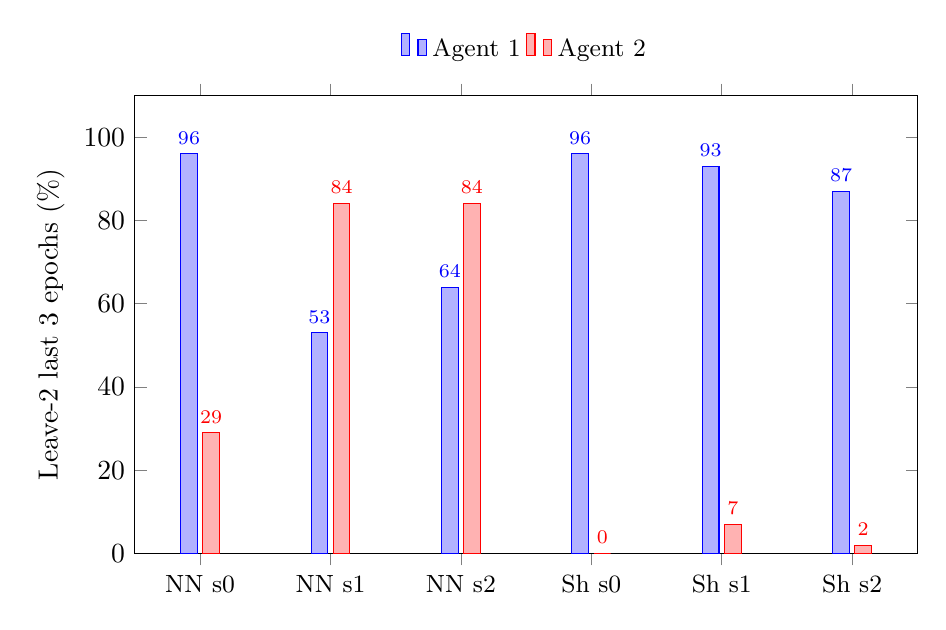
\begin{tikzpicture}
\begin{axis}[
  ybar,
  bar width=6pt,
  width=0.95\textwidth,
  height=7.4cm,
  ylabel={Leave-2 last 3 epochs (\%)},
  ymin=0, ymax=110,
  symbolic x coords={NN0, NN1, NN2, Sh0, Sh1, Sh2},
  xtick=data,
  xticklabels={NN s0, NN s1, NN s2, Sh s0, Sh s1, Sh s2},
  xticklabel style={font=\small},
  legend style={at={(0.5,1.05)}, anchor=south, legend columns=2,
    font=\small, draw=none},
  nodes near coords,
  nodes near coords style={font=\scriptsize, /pgf/number format/fixed},
]
\addplot coordinates {(NN0,96) (NN1,53) (NN2,64) (Sh0,96) (Sh1,93) (Sh2,87)};
\addplot coordinates {(NN0,29) (NN1,84) (NN2,84) (Sh0,0) (Sh1,7) (Sh2,2)};
\legend{Agent 1, Agent 2}
\end{axis}
\end{tikzpicture}
\caption{Share of episodes in the last three epochs that do not open 2.
  NN: centred naive--naive.
  Sh: centred naive--shaper with the extra trial prompt.
  Under naive--naive, which agent leaves 2 swaps across seeds.
  Under naive--shaper, agent 1 leaves 2 and agent 2 does not, on all
  three seeds.
  This figure is that contrast.
  It is not a claim that the shaper taught take-1 and then exploited.}
\label{fig:whodoves}
\end{figure}

It is not a clear shaping success.
This report does not claim that the shaper taught the naive to take 1
and then exploited by taking 2.
Who-doves did not swap under info-on or info-off; it did swap under
matched-LR naive--naive.

\textbf{Slow-LR naive--naive, \(3\times 15\).}
Both episode-update; agent 2 learning rate \(3\times 10^{-7}\).
Last epoch agent 2 opened 2 on \(12/15\) every seed.
Agent 1 leave-2 in the last three epochs: \(78\%\), \(84\%\), \(62\%\);
agent 2: \(33\%\), \(18\%\), \(27\%\).
Who-leaves-2 did not swap.
The same pattern as naive--shaper, without trial update or extra prompt.

Last-epoch returns under naive--naive seed 0 are \(70.7\) and \(75.3\),
near the \(71/72\) open-then-2 split, not the dynamic-program joint
\(210\).
No stock-conditioned 0-then-3 policy appears in last-epoch action
frequencies by stock.

\begin{itemize}
\item \textbf{Grid success (still the bar).}
  The shaper changes the opening distribution or the outcome bins
  relative to centred naive--naive, in a way that tracks the learner's
  current behaviour.
\item \textbf{Grid null.}
  Same openings, same collapse, same bins as the control.
  Live-mix will not rescue a null.
\item \textbf{Not the two-phase claim.}
  Agent 2 leave-2 on the 50-epoch seed was \(25/750\).
  Epoch 1 the shaper opened 2 while the naive still mostly opened 2.
\end{itemize}

\subsection{Noise arm (Stage B)}

Multiplicative \(\xi\in\{0.7,1.0,1.3\}\) on the growth increment.
Numbers below are reported against Table~\ref{tab:noise-dp}.

Pre-fix Test~A \(\xi\) and NN \(\xi\) were not repeated after the
trainer reseed; those two paragraphs are the shared-stream packet.
H3 is given first as that pre-fix family, then as the seed-fixed replica
(NS and slow2).

\textbf{H1--H2, Test~A + \(\xi\) (pre-fix).}
Last-epoch leave-2 is \(98\%\), \(64\%\), \(98\%\)
(openings \(15\times 0\), \(10\times 1+5\times 2\), \(15\times 0\)).
Whole-run survival \(119\), \(41\), \(93\) out of 225; last-epoch
returns \(65.5\), \(26.9\), \(58.3\).
Stage~A centre last openings were \(13\times 1\), \(14\times 1\),
\(14\times 0\).
Against a hawk, opening 0 lands in \(\{9,11,12\}\) and opening 1 in
\(\{8,9,10\}\); constant take-2 thereafter survives with probability
\(0.80\) (return \(58.3\)) from the first set and \(0.40\) (return
\(34.7\)) from the second.
Seeds 0 and 2 moved to the opening that doubles survival, which is also
the sign of \(Q(0)>Q(1)\) under noise.
Their last-epoch returns sit near that \(58.3\) cell; the mixed seed sits
nearer \(34.7\).
Leave-2 at \(R<12\) in the last epoch is \(41\%\), \(28\%\), \(29\%\),
against \(1.00\) for the feedback rule and far below its return \(68.8\).
H1 holds in a stronger form than a mere leave-2 match with Stage~A: two
of three seeds chose the DP-better exit.
H2 is negative: the learner did not learn to condition on stock.

\textbf{Naive--naive + \(\xi\) (pre-fix).}
Survival \(100\), \(43\), \(82\) out of 225; last-epoch returns
\(37.6/45.1\), \(27.9/31.1\), \(48.3/43.8\).
Seed~2 last epoch: agent 1 \(14\times 2\), agent 2 \(13\times 1\)
(leave-2 last3 \(24\%\) / \(87\%\)).
Seed~1 both still mostly opened 2 (survival \(43/225\)), where all three
Stage~A naive--naive seeds had left 2.

\textbf{H3, naive--shaper versus slow2, pre-fix.}
On the shared stream, naive--shaper survival \(90\), \(71\), \(75\) out
of 225; slow2 \(53\), \(44\), \(39\).
Agent 1 leave-2 last3: \(96\%\), \(93\%\), \(89\%\) against the shaper
versus \(69\%\), \(67\%\), \(40\%\) against slow2.
Agent 2 leave-2 last3: \(0\%\), \(11\%\), \(11\%\) (shaper) versus
\(18\%\), \(18\%\), \(20\%\) (slow2).
A more stationary hawk produced a more reliable dove on all three
\emph{nominal} paired seeds.
That agreement is one observation counted three times.

\textbf{H3, seed-fixed, same noise-table pairing, all L40S.}
Seed 0 of each arm is the pre-fix seed-0 tape (opening identity \(1.00\)).
Seeds 1 and 2 are new.
Naive--shaper last3 survival \(36/45\), \(12/45\), \(5/45\); last-epoch
return \(49.7\), \(29.0\), \(12.3\); agent-1 leave-2 last3 \(96\%\),
\(44\%\), \(33\%\); agent-2 leave-2 last3 \(0\%\), \(22\%\), \(22\%\).
Slow2 last3 survival \(21/45\), \(24/45\), \(8/45\); last-epoch return
\(44.8\), \(52.9\), \(13.0\); agent-1 leave-2 last3 \(69\%\), \(76\%\),
\(27\%\); agent-2 leave-2 last3 \(18\%\), \(13\%\), \(22\%\).
Sign of NS minus slow2 on agent-1 leave-2 last3 is \(+\), \(-\), \(+\);
on last-epoch return \(+\), \(-\), \(-\).
Both agent 2s stay mostly on 2.
Learning rate and clip are matched; the remaining difference is the
trial update and the extra prompt.
The 36-unit DP interest in feedback restraint was not collected
(seed-fixed NS leave-2 at \(R<12\) is \(51\%\), \(18\%\), \(27\%\)
for the naive and \(2\%\), \(12\%\), \(5\%\) for the shaper; returns sit
near hawk--dove or collapse, not \(72/68.8\)).
H3 as a shaper-return and more-reliable-dove inequality fails at three
independent seeds.
The pre-fix ``more reliable dove on all three seeds'' does not survive
the replica.
A 50-epoch slow2 \(\xi\) seed 0 continues the 15-epoch snapshot: first
agent-1 majority at epoch 10, last-open \(15\times 0\) versus mixed
agent 2, last-epoch return \(70.5/69.2\), last3 survival \(37/45\).
NS \(\xi\) at 50 epochs was not obtained.

\section{Final grid}
\label{sec:grid-results}

The tables and figures in this section are written by
\texttt{scripts/evaluate\_grid.py} from the records of the final grid
(Chapter~\ref{ch:design}); where a file is absent the arm has not been
run.
\newcommand{\gridinput}[1]{\IfFileExists{tables/grid/#1}{\input{tables/grid/#1}}{\emph{[not yet run: }\texttt{\detokenize{#1}}\emph{]}}}

\subsection{Checks C1 and C2}
\gridinput{B_c2.tex}

\subsection{Stage A: H-A}
\begin{table}[ht]\centering\small
\caption{Stage~A, last-window estimates per arm and seed (interval: Wilson 95\%; return: mean and standard error over the window's games).}
\label{tab:grid-A-arms}
\resizebox{\textwidth}{!}{\gridinput{A_arms.tex}}
\end{table}
\begin{table}[ht]\centering\small
\caption{Stage~A, paired ladder differences \(\Delta_s\) with sign agreement over seeds.}
\label{tab:grid-A-rungs}
\resizebox{\textwidth}{!}{\gridinput{A_rungs.tex}}
\end{table}

\subsection{Stage B: the ladder, H-B1 to H-B4}
\begin{table}[ht]\centering\small
\caption{Stage~B, last-window estimates per arm and seed.}
\label{tab:grid-B-arms}
\resizebox{\textwidth}{!}{\gridinput{B_arms.tex}}
\end{table}
\begin{table}[ht]\centering\small
\caption{Stage~B, paired ladder differences \(\Delta_s\) with sign agreement over seeds.}
\label{tab:grid-B-rungs}
\resizebox{\textwidth}{!}{\gridinput{B_rungs.tex}}
\end{table}
\begin{figure}[ht]\centering
\IfFileExists{figures/grid/B_curves.pdf}{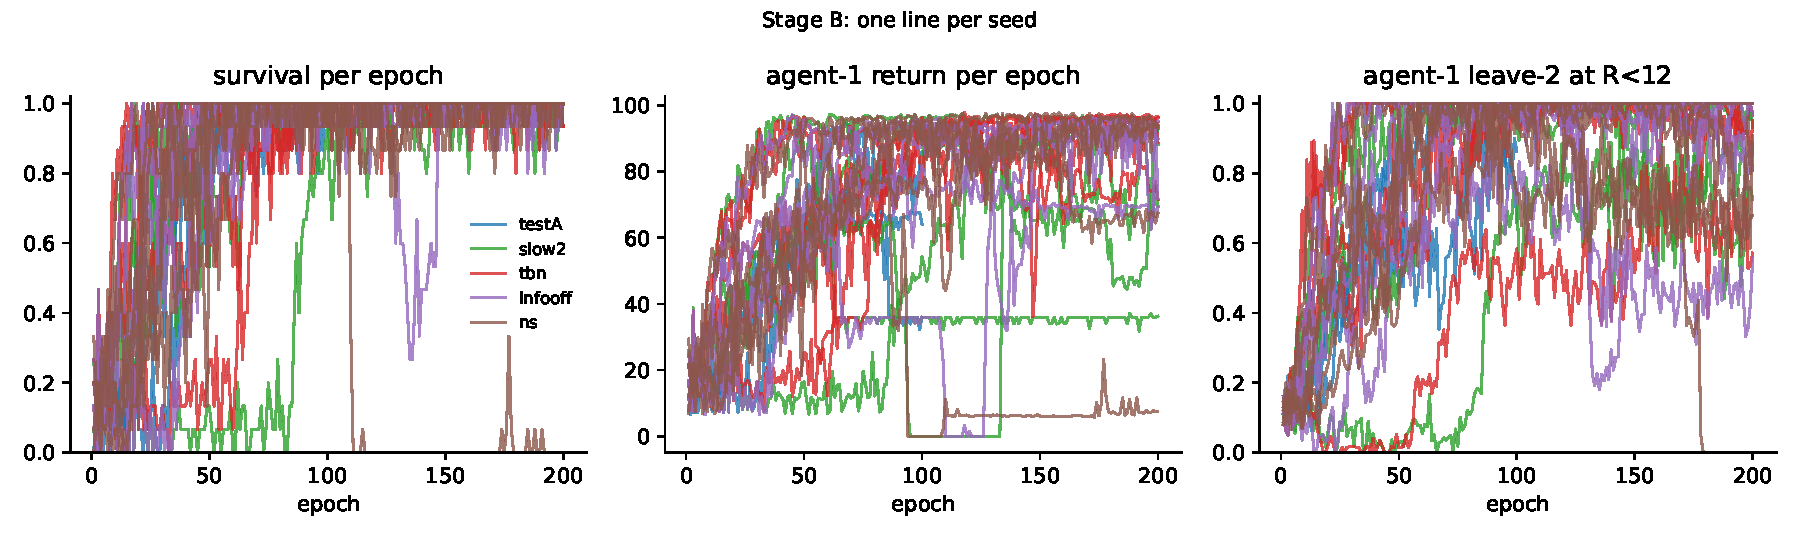
\includegraphics[width=\textwidth]{figures/grid/B_curves.pdf}}{\emph{[not yet run: B\_curves.pdf]}}
\caption{Stage~B learning curves: survival, agent-1 return and agent-1 low-stock restraint per epoch, one line per seed, colour per arm.}
\label{fig:grid-B-curves}
\end{figure}

\subsection{Transfer: H-T}
\gridinput{B_transfer.tex}

\subsection{Sensitivity}
\gridinput{sensitivity.tex}

\chapter{Limitations}
\label{ch:lim}

These constraints limit what the executed contrasts can be said to show.

\section{Wrong efficiency benchmark}

Mutual take-1 returns 36; one \((0,0)\) then mutual 3 returns 105.
Take-3 is the sustainable harvest at high stock.
Language that treats take-3 as smash and take-1 as cooperation is
calibrated to the constant-action reduction, not the dynamic program.
Test~B last-epoch return \(72.4\) is the constant hawk--dove cell, not
the best response \(107\).

\section{Leave-2 is a near-constant-policy statistic}

Opening 2 dies only if the continuer stays on 2.
Opening 0 and opening 1 versus a frozen 2 are different basins
(\(8\to 11\) versus \(8\to 9\)).
Last-epoch action frequencies at \(R=9\) under centred Test~A seed~0 are
about 90~percent take-2.
No executed run learned 0-then-3 as a stock-conditioned policy.

\section{Shaping contrast confounded with learning speed}

A shaper against a learner who only avoids death by opening 1 then
taking 2 has about one unit to gain (\(72\) versus \(71\)).
Slow-LR naive--naive already reproduces who-leaves-2 not swapping,
without trial PPO.

\section{Sample and critic}

Whitened Test~A is a three-seed family, not a law.
Seed~0 last-epoch leave-2 \(2/15\), return \(11.3\), last-three-epoch
survival \(5/45\).
Seeds~1--2 left opening 2 (leave-2 last3 \(87\%\) and \(82\%\); survival
\(97/225\) and \(80/225\)).
Last-epoch counts are out of 15 games.
Matched long naive and shaper-e50 are one seed each.
The value head uses \(\texttt{vf\_coef}=0.01\); opening advantages are
close to return minus a poor baseline.
Centre versus whiten is entangled with that.

\section{Noise}

Integer noise on growth was run (\texttt{noise\_tenths=5}, three centred
Test~A seeds).
Last epoch left 2 via opening 0 on every seed.
Whole-run survival is \(76\), \(140\), \(141\).
That is not a licence to write a growth-noise mechanism.

\chapter{Conclusion}
\label{ch:conc}

This report measured ShapeLLM-style PPO on a two-player logistic chicken
CPR (\(R_0=8\), \(K=40\), \(T=36\), \(\texttt{rate\_tenths}=9\)).
Against a frozen hawk, centre-only advantages left the death-open;
batch whitening did not.
Two centred learners split hawk--dove: who doves swapped under
naive--naive and did not under the shaper configs.
That is not a clear shaping success, and it is not a two-phase teaching
policy.
Stochastic regeneration on the locked update has not been run; a null on
that arm remains reportable.


\appendix
\chapter{Regeneration models: logistic, multiplicative, binomial}
\label{app:binomial}

This appendix derives the deterministic increment of Chapter~\ref{ch:env}
and the Stage~B multiplier of Chapter~\ref{ch:design} from a per-unit
regrowth process, states the renewable-resource models the thesis is
placed against, and reports the exact dynamic-programming values of every
policy in the main text under a third, Pérolat-faithful, regeneration
kernel.
Every number is printed by \texttt{python cpr\_xi.py} and pinned by
\texttt{tests/test\_cpr\_xi.py}.

\section{Per-unit regrowth and its mean field}
\label{app:meanfield}

In Commons Harvest \cite{perolat2017} an empty cell regrows with a
probability that rises with the number of apples nearby and is zero when
none are nearby.
The scalar version of that process on a pool of capacity \(K\) with
escapement (post-harvest stock) \(S\) is: each of the \(K-S\) empty units
regrows independently with probability \(\rho S/K\), so the increment is
\begin{equation}
  \begin{aligned}
  g_{\mathrm{bin}}(S)&\sim\operatorname{Binomial}\!\bigl(K-S,\;\rho S/K\bigr),\\
  \mathbb{E}\,g_{\mathrm{bin}}(S)&=\rho\,\frac{S\,(K-S)}{K},
  \qquad
  \operatorname{Var}g_{\mathrm{bin}}(S)=\rho\,\frac{S\,(K-S)}{K}\Bigl(1-\frac{\rho S}{K}\Bigr).
  \end{aligned}
  \label{eq:binomial}
\end{equation}
The mean is the logistic surplus-production increment of Schaefer
\cite{schaefer1954}, and \eqref{eq:growth} with \(\xi\equiv 1\) is its
rounding to the integers.
The deterministic game of Stage~A is therefore the mean-field limit of the
per-unit process, and Stage~B is a second-moment correction to it: the
multiplier \(\xi_t\in\{0.7,1.0,1.3\}\) preserves the mean of
\eqref{eq:binomial} exactly and adds a bounded, symmetric spread.
Table~\ref{tab:moments} compares the two spreads at the escapement levels
that decide the game.
The binomial spread is proportionally largest at low stock (a coefficient
of variation of \(0.53\) at \(S=4\), against \(0.27\) for \(\xi\)), which
is why the two models differ on the constant-pair cells below.

\begin{table}[ht]
\centering
\caption{Mean and standard deviation of the growth increment at
  escapement \(S\) under the executed \(\xi\) multiplier and under the
  binomial kernel \eqref{eq:binomial}.
  The exact mean is \(\rho S(K-S)/K\); the deterministic increment is its
  half-even rounding.
  \(S=4\) is the escapement under mutual take-2 from \(R_0\); \(S=5\) under
  hawk--dove; \(S=8\) after a symmetric restrained opening or at the joint
  optimum's escapement; \(S=14\) at the joint-optimum stock.}
\label{tab:moments}
\begin{tabular}{rrrrrrr}
\toprule
\(S\) & exact mean & deterministic & \(\xi\) mean & \(\xi\) s.d. & binomial mean & binomial s.d. \\
\midrule
4  & 3.24 & 3 & 3.00 & 0.82 & 3.24 & 1.72 \\
5  & 3.94 & 4 & 4.00 & 0.82 & 3.94 & 1.87 \\
8  & 5.76 & 6 & 5.67 & 1.25 & 5.76 & 2.17 \\
14 & 8.19 & 8 & 8.33 & 2.05 & 8.19 & 2.37 \\
20 & 9.00 & 9 & 9.00 & 2.45 & 9.00 & 2.22 \\
\bottomrule
\end{tabular}
\end{table}

\section{The renewable-resource models}
\label{app:reed}

The discrete-time harvesting model of Reed \cite{reed1979}, in the
notation of Clark \cite{clark1990}, is
\begin{equation}
  X_{t+1}=Z_t\,G(S_t),
  \qquad
  S_t=X_t-h_t,
  \qquad
  Z_t\ \text{i.i.d.},\ \mathbb{E}Z_t=1,
  \label{eq:reed}
\end{equation}
where \(X_t\) is the stock before harvest, \(h_t\) the harvest, \(S_t\)
the escapement, \(G\) a concave stock--recruitment function and \(Z_t\) a
multiplicative recruitment shock.
Reed's result is that the policy maximising expected discounted net
revenue is a constant-escapement rule, \(h_t=\max(0,X_t-S^{*})\), and that
under a self-sustaining condition (the escapement is reachable from every
realised stock) the stochastic optimum \(S^{*}\) coincides with the
deterministic one.
Sethi et al.\ \cite{sethi2005} separate three sources of uncertainty,
growth (\(Z_t\)), measurement (the manager observes \(X_t\) with error) and
implementation (the realised harvest differs from the intended one), and
show that the constant-escapement result survives growth uncertainty alone
but not large measurement or implementation uncertainty.

The game of Chapter~\ref{ch:env} is \eqref{eq:reed} with two harvesters,
\(h_t=a_{1,t}+a_{2,t}\) capped at 3 per player, the Schaefer recruitment
\(G(S)=S+\rho S(K-S)/K\) rounded to the integers, and the shock applied to
the surplus rather than to the whole recruitment:
\begin{equation}
  R_{t+1}=S_t+\xi_t\,g(S_t)
  \qquad\text{instead of}\qquad
  X_{t+1}=Z_t\bigl(S_t+g(S_t)\bigr).
  \label{eq:surplus-shock}
\end{equation}
The difference is deliberate.
Under \eqref{eq:reed} a small \(Z_t\) can take the stock below the
escapement, so collapse can be environmental; under
\eqref{eq:surplus-shock}, since \(\xi_t\ge 0\), the stock never falls below
the escapement and collapse is always a consequence of the players'
requests, which is what makes survival a behavioural statistic.
In Sethi et al.'s taxonomy the thesis studies growth uncertainty only:
the stock is reported to both players exactly every round, and requests
are filled exactly unless the scarcity rule fires.
This is the regime in which Reed's constant-escapement structure survives,
and the dynamic programme confirms it in the two-player game: the joint
optimum of \eqref{eq:bellman-joint} is the constant-escapement policy
``harvest to \(S=8\)'' (one round of \((0,0)\) from \(R_0=8\), then
\((3,3)\) at the fixed point \(R=14\)), and every safe policy of
Table~\ref{tab:noise-dp} is a feedback rule of the same form, constrained
by the per-player cap of 3, which binds below the maximum sustainable
yield of \(\rho K/4=9\).
Reed's model is thus not a form citation for Stage~B; it is the model, with
the shock moved from recruitment to surplus and the harvest split between
two players who do not coordinate.

\section{Dynamic-programming values under the three kernels}
\label{app:dp3}

Table~\ref{tab:dp3} reports every policy of Table~\ref{tab:noise-dp}
under the deterministic increment, the executed \(\xi\) multiplier, and
the binomial kernel \eqref{eq:binomial}.
Under the binomial kernel the constant-pair cells of Table~\ref{tab:chicken}
are no longer invariant: mutual take-2 survives with probability
\(0.17\) and hawk--dove dies with probability \(0.19\), so the opening
incentives of Stage~A would not carry over and the two arms would not be
comparable.
That is the reason the executed Stage~B uses the bounded multiplier
rather than the process it approximates.
The stock-conditioned feedback rules keep their values under all three
kernels (the symmetric rule ``3 if \(R\ge 14\), else 0'' earns
\(102.7\) per player with survival \(1.00\) under both stochastic kernels),
which is the constant-escapement result of Section~\ref{app:reed} in the
two-player game.
The best response to a partner that has learned the feedback rule is
\(107.0\), \(105.5\) and \(104.2\) under the three kernels, against
\(72\) for a hawk that stays on take-2; that gap is the ceiling for what a
shaper could gain by exploiting a partner it has taught to restrain, and
the shaper's return in Chapter~\ref{ch:results} is read against it.

\begin{table}[ht]
\centering
\small
\caption{Expected return per player and survival probability under the
  three regeneration kernels.
  ``Hawk'' is the frozen always-2 partner of Test~A.
  The \(\xi\) column is the executed Stage~B; the binomial column is the
  Pérolat-faithful reference of \eqref{eq:binomial}.
  Exact backward induction, rounded to one decimal; \((1,1)\) under the
  binomial kernel survives with probability \(0.999\).}
\label{tab:dp3}
\resizebox{\textwidth}{!}{%
\begin{tabular}{lcccccc}
\toprule
 & \multicolumn{2}{c}{Deterministic} & \multicolumn{2}{c}{\(\xi\in\{0.7,1,1.3\}\)} & \multicolumn{2}{c}{Binomial} \\
\cmidrule(lr){2-3}\cmidrule(lr){4-5}\cmidrule(lr){6-7}
Policy pair & Return & Survival & Return & Survival & Return & Survival \\
\midrule
\((1,1)\) throughout & 36 / 36 & 1.00 & 36.0 / 36.0 & 1.00 & 36.0 / 36.0 & 1.00 \\
\((2,2)\) throughout & 7 / 7 & 0.00 & 7.4 / 7.4 & 0.00 & 18.1 / 18.1 & 0.17 \\
\((2,1)\) hawk versus dove & 72 / 36 & 1.00 & 72.0 / 36.0 & 1.00 & 60.6 / 30.3 & 0.81 \\
\midrule
\((1,1)\) once, then \((2,2)\) & 71 / 71 & 1.00 & 59.3 / 59.3 & 0.80 & 51.6 / 51.6 & 0.68 \\
Hawk versus ``1 once, then 2'' & 72 / 71 & 1.00 & 35.7 / 34.7 & 0.40 & 35.3 / 34.3 & 0.42 \\
Hawk versus ``0 once, then 2'' & 72 / 70 & 1.00 & 60.3 / 58.3 & 0.80 & 52.6 / 50.6 & 0.68 \\
\((0,0)\) once, then \((3,3)\) & 105 / 105 & 1.00 & 38.6 / 38.6 & 0.25 & 46.3 / 46.3 & 0.36 \\
\midrule
Hawk versus ``1 if \(R<12\), else 2'' & 72 / 69 & 1.00 & 72.0 / 68.8 & 1.00 & 60.6 / 56.9 & 0.81 \\
Both ``2 if \(R\ge 9\), else 1'' & 71 / 71 & 1.00 & 70.8 / 70.8 & 1.00 & 69.7 / 69.7 & 0.99 \\
Both ``3 if \(R\ge 14\), else 0'' & 105 / 105 & 1.00 & 102.7 / 102.7 & 1.00 & 102.7 / 102.7 & 1.00 \\
\midrule
Best response to hawk & 105 & 1.00 & 102.5 & 1.00 & 101.0 & 1.00 \\
Best response to ``1 if \(R<12\), else 2'' & 107 & 1.00 & 105.5 & 1.00 & 104.2 & 1.00 \\
Joint optimum \(W^{*}\) & 210 & 1.00 & 207.1 & 1.00 & 206.3 & 1.00 \\
\bottomrule
\end{tabular}%
}
\end{table}


\bibliographystyle{plain}
\bibliography{refs}

\end{document}
